% ============================================================================
%  Compact Neural Networks for Level-1 Di-Tau Triggering
%  Workshop on Deep Learning (0368-3538-01), Tel Aviv University
%
%  Build: pdflatex main -> bibtex main -> pdflatex main -> pdflatex main
%  (Overleaf does this automatically.)
% ============================================================================
\documentclass{article}

% "preprint" removes line numbers and anonymisation; the footer is replaced below.
\PassOptionsToPackage{numbers,sort&compress}{natbib}
\usepackage[preprint]{neurips_2025}
% Wider text block than the NeurIPS default (6.5in instead of 5.5in, 1in side margins).
\AtBeginDocument{\newgeometry{textheight=9in,textwidth=6.5in,top=1in,headheight=12pt,headsep=25pt,footskip=30pt}}

\usepackage[utf8]{inputenc}
\usepackage[T1]{fontenc}
\usepackage{microtype}
\usepackage{amsmath,amssymb,amsfonts,mathtools}
\usepackage{bm}
\usepackage{siunitx}
\usepackage{booktabs}
\usepackage{float}
\usepackage{capt-of}
\usepackage{placeins}
\usepackage{tabularx}
\usepackage{multirow}
\usepackage{array}
\usepackage{graphicx}
\usepackage{xcolor}
\usepackage{tikz}
\usetikzlibrary{positioning,arrows.meta,fit,calc,shapes.geometric}
\usepackage{enumitem}
\usepackage{hyperref}
\usepackage[capitalize,noabbrev]{cleveref}

\hypersetup{colorlinks=true,linkcolor=blue!55!black,citecolor=blue!55!black,urlcolor=blue!55!black}
\setlist{itemsep=1pt,topsep=2pt,parsep=0pt,leftmargin=1.3em}

% Replace the NeurIPS footer on the first page.
\makeatletter
\renewcommand{\@noticestring}{Workshop on Deep Learning (0368-3538-01), Tel Aviv University, 2026.}
\makeatother

% ---------------------------------------------------------------------------
% Shared notation. Change a symbol here and it changes everywhere.
% ---------------------------------------------------------------------------

% Draft notes. Set \showtodostrue -> \showtodosfalse to hide every note.
\newif\ifshowtodos
\showtodosfalse
\newcommand{\todo}[1]{\ifshowtodos{\color{red!70!black}\textsf{\small[#1]}}\fi}

% Physics quantities
\newcommand{\GeV}{\,\mathrm{GeV}}
\newcommand{\pT}{p_{\mathrm{T}}}
\newcommand{\ptTOB}{p_{\mathrm{T}}^{\mathrm{TOB}}}
\newcommand{\pttruth}{p_{\mathrm{T}}^{\mathrm{true}}}
\newcommand{\tauhad}{\tau_{\mathrm{had}}}
\newcommand{\dR}{\Delta R}

% Trigger quantities
\newcommand{\FPR}{\mathrm{FPR}}
\newcommand{\FPRev}{\mathrm{FPR}_{\mathrm{ev}}}
\newcommand{\FPRtarget}{\varepsilon_{\mathrm{B}}}          % target event FPR (0.005)
\newcommand{\eff}{\epsilon}
\newcommand{\effTOB}{\epsilon^{\mathrm{TOB}}}
\newcommand{\Frac}{\mathrm{Frac}_{\mathrm{EM2}}}
\newcommand{\1}{\mathbf{1}}
\newcommand{\sigmoid}{\sigma}
\newcommand{\E}{\mathbb{E}}

% Sets
\newcommand{\Bset}{\mathcal{B}}   % background events
\newcommand{\Sset}{\mathcal{S}}   % truth-matched tau objects
\newcommand{\Kset}{\mathcal{K}}

% Input bundles (short names used throughout the paper)
\newcommand{\CT}{\textsc{ct}}        % 45 raw core-tensor cells, 5x3x3
\newcommand{\CP}{\textsc{cp}}        % core physics: BDT, pT, deta, dphi
\newcommand{\SUM}{\textsc{sum}}      % 15 per-layer summaries
\newcommand{\Ffeat}{\textsc{f}}      % em2_best_3x3_fraction
\newcommand{\EMtwo}{\textsc{em2}}    % 12x12 EM2 image

% Code identifiers
\newcommand{\code}[1]{\texttt{\small #1}}
\newcommand{\ptTOBof}[1]{p_{\mathrm{T},#1}^{\mathrm{TOB}}}
\definecolor{cbred}{HTML}{E34948}


\hypersetup{pdftitle={TAUminator: Compact Neural Networks for Tau Triggering},
            pdfauthor={Max Golubkov, Tamar Averbuch}}

\newcommand{\repourl}{https://github.com/Maxgolu/Tau-Trigger-NN}
\newcommand{\tauaffil}{{\small\href{https://en.cs.tau.ac.il/computer}{\color{black}Blavatnik School of Computer Science and AI}}}

% Title with the image on the left, between the two title rules.
% To go back to the TikZ emblem, replace the \includegraphics line with % Title emblem: an original "tau on a trigger chip" icon (TikZ, no external image).

\begin{tikzpicture}[x=1cm,y=1cm,line cap=round]
  \definecolor{embdark}{HTML}{184F95}
  \definecolor{embmid}{HTML}{2A78D6}
  \definecolor{emblight}{HTML}{CDE2FB}
  % pins on the four sides
  \foreach \p in {-0.42,-0.14,0.14,0.42} {
    \draw[embdark, line width=1.3pt] (\p,0.62) -- (\p,0.80);
    \draw[embdark, line width=1.3pt] (\p,-0.62) -- (\p,-0.80);
    \draw[embdark, line width=1.3pt] (0.62,\p) -- (0.80,\p);
    \draw[embdark, line width=1.3pt] (-0.62,\p) -- (-0.80,\p);
  }
  % chip body
  \fill[embdark, rounded corners=3pt] (-0.64,-0.64) rectangle (0.64,0.64);
  \draw[embmid, line width=0.8pt, rounded corners=2pt] (-0.54,-0.54) rectangle (0.54,0.54);
  % small calorimeter grid in the corner (3x3 towers)
  \foreach \i in {0,1,2} \foreach \j in {0,1,2}
    \fill[emblight!70] (0.20+0.095*\i,-0.47+0.095*\j) rectangle ++(0.075,0.075);
  \fill[white] (0.295,-0.375) rectangle ++(0.075,0.075);
  % the tau
  \node[text=white, font=\fontsize{30}{30}\selectfont\bfseries] at (-0.06,0.07) {$\boldsymbol{\tau}$};
\end{tikzpicture}
.
\newlength{\emblemwidth}
\setlength{\emblemwidth}{2.2cm}
\title{%
  \begin{tabular}{@{}m{\emblemwidth}@{\hspace{1em}}m{0.66\linewidth}@{\hspace{1em}}m{\emblemwidth}@{}}
    
\includegraphics[width=\emblemwidth]{figures/title_image.jpg} &
    \centering {\huge TAUminator:}\par\vspace{5pt}{\Large Compact Neural Networks for Tau Triggering} &
    \mbox{}
  \end{tabular}%
}

\author{%
  Max Golubkov \\
  \tauaffil \\
  Tel Aviv University \\
  \texttt{maximg@mail.tau.ac.il} \\
  \And
  Tamar Averbuch \\
  \tauaffil \\
  Tel Aviv University \\
  \texttt{averbuch2@mail.tau.ac.il} \\
}

\begin{document}

\maketitle

% ============================================================================
\section{Introduction}
\label{sec:intro}
% ============================================================================
Identifying tau particles is important in studies of particles such as the
Higgs and Z bosons. Many taus decay into a narrow spray of particles, which
leaves a compact energy deposit in the ATLAS calorimeter. Ordinary jets of
particles can leave a similar deposit, especially at low energy. A simple
energy threshold therefore either accepts too much background or rejects useful
tau candidates.

The decision must be made while collision data are arriving. The Large Hadron
Collider (LHC) produces proton collisions at \SI{40}{MHz}, far faster than
ATLAS can store them. Its first-stage, or Level-1, trigger therefore keeps only
a small fraction for later reconstruction~\cite{atlas_trigger_run3,atlas_phase1_tdr}.
We study compact neural networks for the calorimeter Trigger Objects (TOBs)
supplied by the electron Feature Extractor (eFEX). The comparison is made at a
fixed event fake rate of $0.5\%$: a useful model must retain more signal without
accepting more background events.

We first study models that score one TOB at a time. We test which detector
inputs carry useful information, whether compact convolutional networks improve
on fully connected networks, and how the classifier and loss can protect the required efficiency
across the energy range. We then ask a different question: can the network make
a better event decision if it sees two TOBs together? The pair model applies
the same small network to both TOBs, scores every pair in the event and uses the
highest pair score. During training, every event receives equal weight even
when it contains many pairs.

For the single-TOB study, the strongest global model accepts $69.61\%$ of
truth-$\tau$ objects, compared with $57.37\%$ for the eFEX baseline. The
pair study uses a different measure: the fraction of signal events that fire.
On its final test, this efficiency rises from $34.30\%$ for the second-highest-
$\ptTOB$ baseline to $46.70\%$, a gain of 12.40 percentage points. The three
models reach event fake rates of $0.5183$--$0.5223\%$, slightly above the
$0.5\%$ limit. The efficiency improvement is therefore clear, but the final
success criterion is not met. The two studies use different denominators and
their percentages should not be compared directly.

\noindent\textbf{Code and demo:} \url{\repourl}

% ============================================================================
\section{Background and Related Work}
\label{sec:background}
% ============================================================================

\paragraph{Why the trigger must filter, and why at a fixed rate.}
The LHC collision rate is \SI{40}{MHz}, far beyond readout capacity. The FPGA-based Level-1 trigger selects about \SI{100}{kHz} within a few microseconds~\cite{atlas_trigger_run3}, using fast detector inputs; eFEX supplies calorimeter trigger objects (TOBs)~\cite{atlas_phase1_tdr}. Our di-tau selection is assigned a $0.5\%$ background-event acceptance budget. The relevant comparison is therefore \emph{signal efficiency at the same background rate}, not threshold-free ROC-AUC (\cref{sec:setting}; trigger context in \cref{app:trigger_context}).

\paragraph{The tau particle and why it is hard to trigger on.}
A tau is a short-lived relative of the electron, produced in processes such as Higgs and $Z$ decays. It decays before reaching the detector. We target its hadronic decays (about $65\%$~\cite{pdg2024}), whose particles leave narrow energy deposits, or \emph{showers}, in the calorimeter. The challenge is that far more common QCD jets can produce similar deposits, especially at low energy. A loose energy cut admits too many jets; a tight cut loses low-energy taus. We therefore use shower shape as well as energy to distinguish them (\cref{app:tau_context}).

\paragraph{Calorimeter inputs.}
Each TOB has a $5\times3\times3$ core tensor spanning four electromagnetic layers (EM0--EM3) and one hadronic layer~\cite{atlas_detector}, plus a finer $12\times12$ EM2 view of the same angular region. For example, the real tau candidate with $\ptTOB=\SI{31.2}{GeV}$ in \cref{fig:calo_input} is represented by five $3\times3$ energy maps (45 values) and 144 EM2-bin energies, not by a photograph. Available scalars are $\ptTOB$, position and an eFEX BDT score. Truth quantities supply labels, loss weights and evaluation variables, never inference inputs; \cref{app:data} specifies their construction.

\begin{figure}[t]
  \centering
  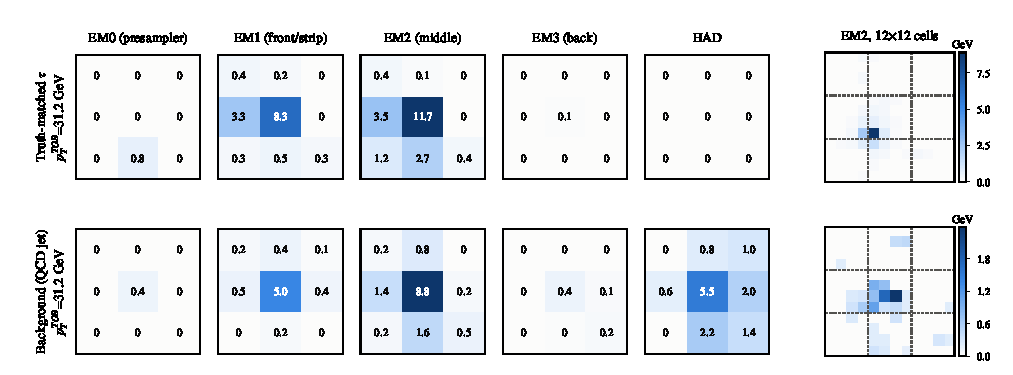
\includegraphics[width=\linewidth]{figures/fig_calo_input.pdf}
  \caption{Calorimeter input of two typical training objects with equal $\ptTOB=\SI{31.2}{GeV}$. Each is chosen at its class median of $\Frac$ (\cref{eq:frac}) and of deposited energy per unit $\ptTOB$. Left: the five $3\times3$ core layers (GeV). Right: EM2 at $12\times12$ granularity; dashed lines mark the towers. The one-prong $\tau$ ($\pttruth=\SI{42.7}{GeV}$) is compact, lies in EM1--EM2 and has no hadronic energy. The jet is wider and deposits much of its energy in HAD.}
  \label{fig:calo_input}
\end{figure}

\paragraph{Prior work.}
This project continues the study of Kernan and Areva Cohen~\cite{kernan2026}, carried out with physicists of the group. They designed physically motivated shower features: per-layer energy sums, core dominance and sparsity (\cref{app:layer_summaries}), and EM2 shape variables such as maxima, peak distances and widths (\cref{app:em2_features}). They then tested how well a $[32,16]$ MLP trained with BCE learns from them. EM1 and EM2 carried most of the separating power, and larger MLPs did not help. Their strongest configuration is shown separately in \cref{fig:results_main}b because its evaluation protocol differs.
On related simulations, \citet{yaari2025trees} compared boosted trees, small MLPs and ResNet-style CNNs for Level-1 $\tau$ selection; the ResNets did not fit the FPGA resources. Tools such as \texttt{hls4ml}~\cite{duarte2018hls4ml} make small fixed-latency networks deployable.

\paragraph{CNNs for detector images.}
Compact convolution--pooling stacks can beat much larger ResNets at low false-positive rates~\cite{ayyar2020cnn}. IceCube uses separate input branches for detector regions of different granularity~\cite{icecube2025cnn}, and strided convolutions can serve as a learned down-sampling front end~\cite{kim2023hotspots}. These ideas shaped our designs in \cref{sec:arch}.

\paragraph{Learning at a fixed operating point.}
Efficiency at a fixed fake rate is a \emph{non-decomposable} objective, because the threshold is itself a quantile of the scores. Such objectives can be optimised with Lagrangian relaxations~\cite{eban2017scalable}. With non-differentiable rate constraints, one can train on smooth surrogates and enforce the constraints from the true rates~\cite{cotter2019proxy}. Our constrained loss (\cref{sec:loss}) follows this separation.

% ============================================================================
\section{Experimental Setting}
\label{sec:setting}
% ============================================================================

\paragraph{Data.}
We use Monte Carlo $\tau$-signal and QCD dijet-background samples from the resimulated FEX truth/all-cell production, with detector-level inputs and generator-level truth. Per event, we retain up to the six highest-$\ptTOB$ tau Trigger Objects (TOBs) from the simulated Level-1 Electron Feature Extractor (eFEX), discarding events without TOBs. A signal-sample TOB is positive if its closest visible truth $\tau$ satisfies $\Delta R<0.15$; all other TOBs are negative. The inputs described in \cref{sec:background} are binned within a $0.3\times0.3$ $(\eta,\phi)$ window around each TOB. The retained dataset contains $72{,}404$ signal and $249{,}022$ background events, $1.81$M objects and $110{,}921$ matched $\tau$ objects. For each of three seeds, complete events are randomly split $70/10/20\%$ into training, validation and test sets; grouping by (sample, event number) prevents event leakage and identifier collisions. Sample identifiers, input construction and split statistics are given in \cref{app:data}.

\paragraph{Event decision and calibration.}
A model assigns every object $i$ of event $e$ a score $s_{e,i}=f_\theta(x_{e,i})$, computed from that object's inputs $x_{e,i}$. An object is accepted when $s_{e,i}\geq t$, and the event fires when at least two objects are accepted (\cref{fig:arch}b):
\begin{equation}
  A_e(t)=\1\Big[\textstyle\sum_i\1[s_{e,i}\geq t]\geq2\Big]=\1\big[s_{e,(2)}\geq t\big],
  \label{eq:event_decision}
\end{equation}
where $s_{e,(2)}$ is the second-highest object score in event $e$. The \emph{event-level} fake rate $\FPRev(t)$ is the fraction of background events $\Bset$ that fire. It is not the fraction of background objects. The threshold is the lowest score value that keeps the fake rate within the budget:
\begin{equation}
  t^\star=\min\big\{t\in\{s_{e,(2)}\}_{e\in\Bset}:\FPRev(t)\leq\FPRtarget\big\},\qquad\FPRtarget=0.005 .
  \label{eq:calibration}
\end{equation}
The search runs over the unique score values, so tied scores are never split, and deployment uses the same $\geq$ comparison. A discrete score may therefore reach only a fake rate below $0.5\%$, so we always report the \emph{achieved} rate (\cref{app:calibration}).

\paragraph{Metrics and baseline.}
Signal efficiency is the fraction of truth-$\tau$ objects accepted, reported versus true $\pT$ (the \emph{turn-on}) and globally. The baseline accepts objects with $\ptTOB\geq C$ under the same two-object event rule. For fixed-rate comparisons, both are recalibrated on the same test background at $0.5\%$; achieved rates are reported, while validation-calibrated performance is a separate transfer check. The goal is earlier turn-on without sacrificing efficiency above $\SI{25}{GeV}$. Reporting bands, baseline response and calibration distinctions are detailed in \cref{app:metric_protocol}.

\paragraph{Hardware constraints.}
An indicative FPGA budget of about $4{,}000$ 8-bit weights, together with changing input and operation constraints, motivated a range of compact candidates rather than one hardware-specific optimum. We compare roughly $2$k-parameter MLPs, $4$--$5$k EM2-only CNNs and $9$k dual-branch CNNs. Counts include BatchNorm; parameter count alone does not establish hardware feasibility (\cref{app:hardware_scope}).

\paragraph{Training and selection.}
Inputs are standardised on training data. BCE-based training uses Adam~\cite{kingma2015adam} ($10^{-3}$, batch size $256$, $20$ epochs); results average three seeds. We \emph{select for the trigger, not for BCE}: each epoch is calibrated on validation background and ranked by validation efficiency or the configured trigger objective at $\FPRtarget$. Minimum-BCE checkpoints remain references. Test data do not select features, losses, budgets, architectures or checkpoints. Sweeps, fine-tuning settings and selection details appear in \cref{app:training,app:constrained}.

% ============================================================================
\section{Methodology}
\label{sec:method}
% ============================================================================
To support the changing hardware requirements of \cref{sec:setting}, we studied four complementary axes: data and features (\cref{sec:features}), classifier and loss (\cref{sec:loss}), architecture (\cref{sec:arch}) and the input unit (\cref{sec:input_unit}). Matched comparisons isolate individual mechanisms where possible. Models are named by their inputs, architecture and training objective; \cref{tab:naming} (\cref{app:naming}) explains every name.

% ----------------------------------------------------------------------------
\subsection{Data exploration and feature engineering}
\label{sec:features}
% ----------------------------------------------------------------------------
We compared class-normalised distributions of $\tau$ and non-$\tau$ objects on the training split, overall and within the $\ptTOB$ intervals $[5,10)$, $[10,20)$, $[20,40)$, $[40,80)$ and $[80,120)\GeV$. A variable carries information beyond energy only if the classes still differ \emph{inside} each interval. All features live in a modular registry and are selected by configuration (\cref{app:features}).

\paragraph{Energy: a strong separator and a shortcut.}
$\ptTOB$ is the strongest single separator (\cref{fig:features}a). Non-$\tau$ objects pile up at the $\SI{5}{GeV}$ threshold, while $\tau$ objects have a long tail. For the same reason it is a \emph{shortcut}: a network trained with BCE lowers its loss by learning the energy scale and has little incentive to learn the weaker, complementary shape information. This observation motivated the classifier of \cref{sec:loss}.

\paragraph{EM2 compactness.}
The most useful engineered variable is the fraction of the $12\times12$ EM2 energy contained in its most energetic $3\times3$ cell window:
\begin{equation}
  \Frac=\max_{w\in\mathcal{W}}\sum_{(a,b)\in w}E_{ab}\Big/\sum_{a,b}E_{ab},
  \label{eq:frac}
\end{equation}
where $\mathcal{W}$ is the set of the $100$ overlapping $3\times3$ windows (\cref{fig:features}c,d). A cell window is smaller than one tower, so $\Frac$ measures compactness at a granularity the core tensor cannot resolve. Unlike $\ptTOB$, its separation persists within fixed energy intervals and grows with energy (\cref{fig:features}b, \cref{fig:frac_conditioned}).

\begin{figure}[t]
  \centering
  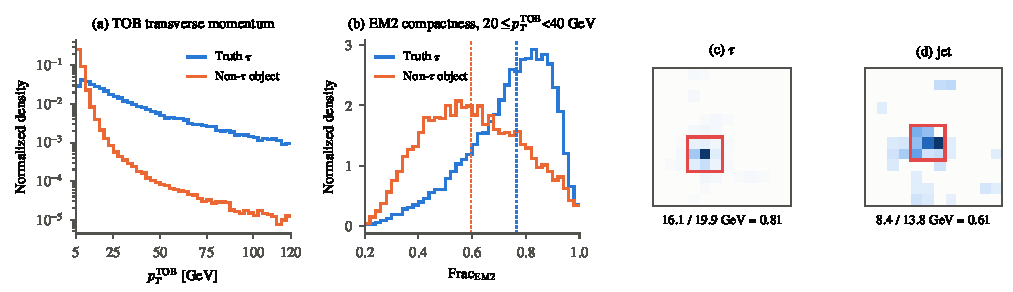
\includegraphics[width=0.95\linewidth]{figures/fig_features.pdf}
  \caption{Feature study (training split, normalised per class). (a) $\ptTOB$, log scale. (b) $\Frac$ for $20\leq\ptTOB<\SI{40}{GeV}$; dashed lines mark the medians. (c,d) Computation of $\Frac$ for the objects of \cref{fig:calo_input}: the red square is the best $3\times3$ window.}
  \label{fig:features}
\end{figure}

\paragraph{Inputs used below.}
Besides $\Frac$ (\Ffeat), four inputs stayed competitive at the operating point:
the 45 raw core cells (\CT), the strongest single input throughout;
15 per-layer summaries (\SUM), which are the sum $S_\ell$, the dominance $2M_\ell-S_\ell$ ($M_\ell$ the maximum cell) and the sparsity $\#\{\text{cells}>0.1M_\ell\}$ of each layer~\cite{kernan2026};
the ``core physics'' vector (\CP): BDT score, $\ptTOB$, and $\eta,\phi$ relative to the leading TOB;
and the EM2 image, which only the CNNs read.
Event-topology variables (the $\ptTOB$ sum, the second-highest $\ptTOB$, the separation of the two leading TOBs) clearly separate events by $\tau$ multiplicity. However, they take the same value for every object of an event, cannot rank the objects within it, and did not improve on object-level inputs at $\FPRtarget$ (\cref{sec:input_unit}, \cref{app:features}).

% ----------------------------------------------------------------------------
\subsection{Classifier and loss design}
\label{sec:loss}
% ----------------------------------------------------------------------------
BCE measures the average quality of object-level probabilities. The trigger instead depends on the far tail of the \emph{event-level} background distribution and has explicit requirements per energy region. We addressed this mismatch in three steps, each changing one mechanism: the decision rule, the signal weighting and the training objective.

\paragraph{The TOB--NN OR classifier.}
Instead of asking a network to relearn the energy threshold, we pair it with the deterministic TOB comparator: accept an object through either branch, then require two accepted objects per event,
\begin{equation}
  a_{e,i}=\1[\ptTOBof{e,i}\geq C]\vee\1[s_{e,i}\geq t],\qquad A_e=\1\Big[\textstyle\sum_i a_{e,i}\geq2\Big].
  \label{eq:or}
\end{equation}
The TOB branch protects the high-energy plateau; the NN supplies complementary shape-based decisions. Thresholds are calibrated jointly, counting mixed-branch events exactly. Validation selects the TOB budget $b$ to maximise the equally weighted efficiency gain across $25$--$100\GeV$, subject to the event fake-rate limit and regional protection guards. A smaller selected $b^\star$ suggests less reliance on the comparator, not a standalone measure of NN quality. Training remains (weighted) BCE; the OR changes the decision rule only. \Cref{app:or} gives the objective, cross-fitted calibration, guards and earlier two-expert trial.

\paragraph{Spectrum-aware signal weighting.}
We reweight each object's contribution to binary cross-entropy:
\begin{equation}
  \mathcal L_{\mathrm{wBCE}}=-\frac1N\sum_i w_i\big[y_i\log s_i+(1-y_i)\log(1-s_i)\big],
  \label{eq:weighted_bce}
\end{equation}
where $y_i$ is the signal label and $s_i$ the NN score. Background keeps $w_i=1$; for signal, $w_i=r(t_i)/\langle r\rangle_{\mathrm{train},S}$, with truth momentum $t_i$ in GeV. Mean-one normalisation preserves the total signal weight while redistributing its gradient across energies. We compare two raw profiles:
\begin{equation}
  \begin{aligned}
    r_{\mathrm{IF}}(t)&=\operatorname{clip}\!\left(\bar n/n_{k(t)},\,0.2,\,5\right),
    & r_p(t)&=\operatorname{clip}(t,10,200)^{-p}.
  \end{aligned}
  \label{eq:powerlaw}
\end{equation}
\emph{Inverse frequency} (IF) uses the training-signal count $n_k$ in each populated $5\GeV$ bin over $25$--$100\GeV$, with $\bar n$ their mean; outside these bins, $r_{\mathrm{IF}}=1$. Rare bins receive larger weights, approximately balancing their total influence. \emph{Power-law weighting} varies smoothly: $p=-1$ doubles the weight when energy doubles away from the clamp, whereas $p=0$ recovers BCE. Since soft taus dominate the sample, both IF and negative $p$ shift learning towards rarer, cleaner energetic examples without resampling the data. This often helped more than further emphasising ambiguous low-energy taus, but depended on the inputs. Full profiles, scans and the transfer hypothesis appear in \cref{app:weighting}; comparisons are in \cref{app:analysis_weighting}.

\paragraph{A constrained trigger objective.}
A fixed weight profile applies the same emphasis whether or not a protection is at risk. Our last step therefore optimises the trigger objective itself. It had a second, more general aim: to find out what a loss that truly represents the trigger problem must look like, and which properties it must have. We collect these conclusions in \cref{sec:lessons}. The problem is
\begin{equation}
  \max_\theta\sum_{k\in\Kset_J}w_k\big[\eff_k(\theta)-\effTOB_k\big]\quad\text{s.t.}\quad\FPRev(\theta)\leq\FPRtarget,\;\;\eff_k(\theta)\geq r_k\;\;(k\in\Kset_C).
  \label{eq:constrained}
\end{equation}
The Lagrangian rewards turn-on gains while penalising fake-rate and regional
deficits. Training uses smooth decisions; exact out-of-sample checks,
threshold recalibration, temperature annealing and uncertainty-aware
fine-tuning stabilise the optimisation (\cref{app:constrained}).

% ----------------------------------------------------------------------------
\subsection{Architectures}
\label{sec:arch}
% ----------------------------------------------------------------------------
Every model in this paper is assembled from the same parts (\cref{fig:arch}a). Optional convolutional branches read the core tensor and the EM2 image, their outputs are concatenated with scalar inputs, and a $[32,16]$ dense head produces the object score. The model names in \cref{tab:naming} describe which parts are used.

\paragraph{MLP.}
The reference model is the $[32,16]$ ReLU MLP with a sigmoid output of~\cite{kernan2026}. On the 45 core cells plus $\Frac$ (\CT+\Ffeat, 46 inputs) it has $2{,}049$ parameters. Larger MLPs did not help~\cite{kernan2026}, so we looked for a better inductive bias rather than more capacity.

\paragraph{Convolutions on the core tensor.}
A flat MLP must learn from data that neighbouring cells are adjacent. A convolution builds in locality and weight sharing instead. Many hand-made features are in fact fixed convolutions followed by pooling; $\Frac$, for example, is an all-ones $3\times3$ kernel, a global maximum and a division. We tested four backbones on the $5\times3\times3$ tensor. V1 mixes the five layers at every cell ($1\times1\times5$ kernel) and learns longitudinal profiles. V2 learns local spatial patterns ($2\times2\times5$ kernel). V3 applies them in series, and V4 in parallel. Because the window is centred on the TOB seed, position matters, so the maps are flattened rather than pooled. \Cref{app:vbackbones} explains each backbone step by step, and \cref{fig:cnn_blocks}a draws them.

\paragraph{A branch for the full-granularity EM2 layer.}
Following~\cite{ayyar2020cnn,icecube2025cnn,kim2023hotspots}, the $12\times12$ EM2 image gets its own branch. E1 applies one $3\times3$ convolution with four filters and $2\times2$ max pooling. E2 adds a second convolution block. E3 learns its down-sampling with a stride-2 convolution. The \emph{dual-branch} model concatenates a V-backbone, an E-branch and optionally $\Frac$ into one head. \Cref{app:ebranches} and \cref{fig:cnn_blocks}b give the details.

\paragraph{Is $\Frac$ still needed next to the EM2 branch?}
Although $\Frac$ is derived from EM2, a small CNN need not learn its global normalisation easily. We therefore compare matched models with and without the scalar: does an explicit scale-free ratio complement learned local patterns? The ablation is reported in \cref{app:analysis_representation}; the architectural rationale is in \cref{app:fraction_complementarity}.

\paragraph{Towards a smaller model: EM2 only.}
EM2's strong contribution motivated removing the core convolution, but not the core measurements: the 45 cells or 15 layer summaries enter the dense head as scalars beside the E-branch and $\Frac$. This tests whether spatial processing is worth its parameter cost (\cref{app:em2only,app:analysis_representation}).

\paragraph{Stability and simplicity.}
Every convolution is followed by BatchNorm~\cite{ioffe2015batchnorm} and LeakyReLU~\cite{maas2013leaky}, which keeps training stable on this highly imbalanced data. Inputs are standardised energies (\cref{app:arch}). Their performance is compared in \cref{sec:analysis}. All parameter counts are listed in \cref{tab:params}.

\begin{figure}[t]
  \centering
  \resizebox{0.95\linewidth}{!}{% Architecture and event-decision diagram (TikZ). Included from Sec. 4.3.
\definecolor{archblue}{HTML}{2A78D6}
\definecolor{archorange}{HTML}{EB6834}
\definecolor{archink}{HTML}{52514E}
\begin{tikzpicture}[
  font=\scriptsize,
  >={Stealth[length=1.4mm]},
  box/.style={draw=archink, rounded corners=1.5pt, align=center, inner sep=1.8pt, line width=0.4pt, minimum height=6.5mm},
  inp/.style={box, fill=archblue!7, text width=15mm},
  conv/.style={box, fill=archblue!22, text width=20mm},
  dense/.style={box, fill=archink!10},
  acc/.style={box, fill=archorange!14, text width=23mm, minimum height=5mm},
  obj/.style={box, fill=archblue!7, minimum width=6mm, minimum height=5mm},
  arr/.style={->, draw=archink, line width=0.45pt},
  lbl/.style={font=\footnotesize\bfseries},
  note/.style={font=\tiny, text=archink, align=center}
]
% ---------------- (a) single-object model ----------------
\node[lbl] at (-0.55,1.25) {(a)};
\node[inp]  (ct)   at (0.25, 0.75) {core tensor\\$5\times3\times3$};
\node[inp]  (em2)  at (0.25,-0.15) {EM2 image\\$12\times12$};
\node[inp, minimum height=5mm]  (frac) at (0.25,-0.95) {$\Frac$};
\node[conv] (ctb)  at (2.45, 0.75) {backbone V1--V4\\(layer mix / spatial)};
\node[conv] (emb)  at (2.45,-0.15) {branch E1--E3\\(conv, pool / stride)};
\node[circle, draw=archink, inner sep=0.5pt, line width=0.4pt] (cat) at (4.05,0.30) {$\oplus$};
\node[dense, text width=14mm] (head) at (5.05,0.30) {dense $[32,16]$\\+ sigmoid};
\node (s) at (6.3,0.30) {$s_{e,i}$};
\draw[arr] (ct) -- (ctb);
\draw[arr] (em2) -- (emb);
\draw[arr] (ctb.east) -- (cat);
\draw[arr] (emb.east) -- (cat);
\draw[arr] (frac.east) -| (cat.south);
\draw[arr] (cat) -- (head);
\draw[arr] (head) -- (s);
\node[note] at (2.45,1.30) {conv\,$\to$\,BatchNorm\,$\to$\,LeakyReLU};
% ---------------- (b) event decision ----------------
\begin{scope}[xshift=7.25cm]
\node[lbl] at (-0.35,1.25) {(b)};
\foreach \k/\y in {1/0.88,2/0.25,3/-0.38} {
  \node[obj] (x\k) at (0.1,\y) {$x_{e,\k}$};
  \node[dense, minimum height=5mm] (f\k) at (0.95,\y) {$f_\theta$};
  \node[acc] (a\k) at (2.7,\y) {$s_{e,\k}\!\ge\! t\;\vee\;q_{e,\k}\!\ge\! C$};
  \draw[arr] (x\k) -- (f\k);
  \draw[arr] (f\k) -- (a\k);
}
\node at (0.1,-0.78) {$\vdots$};
\node at (0.95,-0.78) {$\vdots$};
\node at (2.7,-0.78) {$\vdots$};
\node[note] at (0.5,-1.15) {shared weights, $\leq6$ TOBs};
\node[box, fill=archblue!22, minimum height=6mm] (cnt) at (4.95,0.25) {$\sum_i a_{e,i}\geq2$};
\node (Ae) at (6.2,0.25) {$A_e$};
\foreach \k in {1,2,3} { \draw[arr] (a\k.east) -- (cnt.west); }
\draw[arr] (cnt) -- (Ae);
\node[note] at (4.95,-0.42) {calibrated to\\$\FPRev\leq0.5\%$};
\end{scope}
\end{tikzpicture}
}
  \caption{Overview of the single-object pipeline. (a) How every model is assembled: optional convolutional branches on the core tensor (V1--V4) and on the EM2 image (E1--E3), concatenated with scalar inputs such as $\Frac$, feed a $[32,16]$ head. The MLP uses flat inputs only. (b) How object scores become an event decision (\cref{sec:setting,sec:input_unit}): one shared network scores every TOB; the OR classifier also accepts an object when $q_{e,i}=\ptTOB\geq C$; the event fires with at least two accepted objects.}
  \label{fig:arch}
\end{figure}

% ----------------------------------------------------------------------------
\subsection{Input unit: single-object and pair-object models}
\label{sec:input_unit}
% ----------------------------------------------------------------------------
\paragraph{Single-object models.}
All models above score each TOB independently, with one shared network applied to that object's inputs. The event decision is taken afterwards by the counting rule~\eqref{eq:event_decision} or by the OR rule~\eqref{eq:or} (\cref{fig:arch}b). The decision is therefore independent of TOB order. One small circuit can be replicated for every TOB slot. Training uses object labels, while calibration and evaluation are done at event level. The price is that the network sees no event context: an event-level input is identical for all objects of an event, so it cannot rank them.

\paragraph{Pair-object models.}
We score every unordered pair of finite-$\ptTOB$ TOBs from the same event.
Both members use the same encoder; the complete model has $4{,}357$ parameters.
Its inputs are the
fine EM2 image, coarse cells, measured $\ptTOB$, $\Frac$ and event context.
Same-label pairs teach the model; inference scores all pairs. Training averages
weighted BCE within each eligible event, then averages those event losses.
This removes extra weight from pair multiplicity; signal weights still vary.
Details and \eqref{eq:pair_event_loss} appear in \cref{app:pair_protocol}.

The neural event score is $s_e=\max_{(i,j)\in\mathcal P_e}s_{e,ij}$;
$q_e$ is the second-highest finite $\ptTOB$. The joint decision is
\begin{equation}
  A_e=\1[s_e\geq t]\vee\1[q_e\geq C].
  \label{eq:pair_decision}
\end{equation}
Both branches share one event-level background budget. Checkpoints and
thresholds are selected on validation independently for each training seed;
the models are not combined into an ensemble. Events without a pair receive
a non-passing score and remain in the evaluation denominators.

% ============================================================================
\FloatBarrier
\section{Results and Benchmarking}
\label{sec:results}
% ============================================================================
The fixed-rate protocol below applies to the single-object results;
\cref{sec:pair_results} reports the pair model with unchanged validation thresholds.
Our results use the fixed-rate protocol of \cref{sec:setting}: achieved event fake rates are $0.498$--$0.499\%$, band efficiencies pool tau counts, and entries are three-seed means with standard errors. Checkpoints and OR budgets are selected on validation; test-background recalibration is used only for fixed-rate reporting. Ranking finished configurations is descriptive, not a further unbiased test. The prior-work reference has a different protocol (\cref{app:prior_reference}). \Cref{tab:naming} decodes all model names; IF denotes inverse-frequency weighting, whereas $p$ denotes the separate $t^{-p}$ profile.

% ----------------------------------------------------------------------------
\subsection{Benchmark: performance under different size and plateau requirements}
\label{sec:benchmark}
% ----------------------------------------------------------------------------
\Cref{tab:results_main} selects the highest-global-efficiency model satisfying each row's criterion. \emph{All bands} means that the three-seed mean exceeds the baseline in every reported band, not that every seed does so. These are candidates for hardware evaluation, not validated FPGA implementations.

% Keep the benchmark plot and its table together, after the Section 5 heading.
\begin{figure}[!htbp]
  \centering
  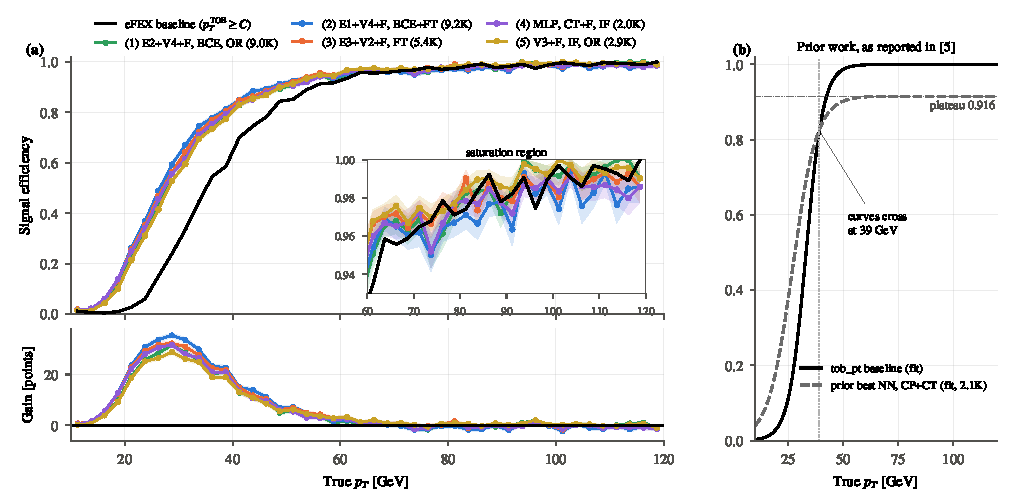
\includegraphics[width=0.97\linewidth]{figures/fig_results_main.pdf}
  \caption{(a) Benchmark turn-ons; model numbers refer to \cref{tab:results_main}. The inset shows saturation, and the lower panel shows gains over the eFEX baseline. Shading indicates statistical uncertainty. (b) Prior-work NN and baseline fits from~\cite{kernan2026}, shown as a separate historical reference. The newly supplied band averages in \cref{tab:results_main} are not point samples of this fit (\cref{app:prior_reference}). Model-name key: \cref{tab:naming}.}
  \label{fig:results_main}
\par\medskip
  \begingroup
  \centering
  \captionof{table}{Benchmark efficiencies [\%] by true-$\pT$ band [GeV]. Red marks our values below the baseline; counts include BatchNorm. The prior-work row is a separately evaluated reference, not part of the ranking. Model-name key: \cref{tab:naming}; provenance: \cref{app:prior_reference}.}
  \label{tab:results_main}
  \small
  \setlength{\tabcolsep}{4pt}
  \begin{tabular}{@{}llrrrrrrr@{}}
\toprule
Criterion & Model & 10--25 & 25--40 & 40--60 & 60--100 & 100--120 & Global & Params \\
\midrule
(1) all bands & E2+V4+\Ffeat, BCE, OR & 14.65 & 62.38 & 88.99 & 97.17 & 99.44 & 67.97$\pm$0.55 & 9.0K \\
(2) global & E1+V4+\Ffeat, BCE+FT & 17.45 & 66.39 & 90.54 & \textcolor{cbred}{96.75} & \textcolor{cbred}{98.28} & 69.61$\pm$0.29 & 9.2K \\
(3) global, $<$6K & E3+V2+\Ffeat, FT & 16.93 & 64.31 & 90.08 & 97.56 & \textcolor{cbred}{98.89} & 69.08$\pm$0.35 & 5.4K \\
(4) global, $<$3K & MLP, \CT+\Ffeat, IF & 16.61 & 62.93 & 89.00 & 97.17 & \textcolor{cbred}{98.53} & 68.40$\pm$0.21 & 2.0K \\
(5) all bands, $<$3K & V3+\Ffeat, IF, OR & 14.13 & 60.42 & 89.14 & 97.89 & 99.50 & 67.47$\pm$0.22 & 2.9K \\
\midrule
--- & Prior best NN, \CP+\CT~\cite{kernan2026} & 12.59 & 60.07 & 86.44 & 90.90 & 91.63 & 62.53 & 2.1K \\
--- & eFEX baseline & 2.28 & 35.85 & 81.60 & 96.89 & 99.34 & 57.37 & --- \\
\bottomrule
\end{tabular}

  \endgroup
\end{figure}

The practical trade-off is clear: all five models turn on earlier, but the highest global efficiency, strongest plateau and smallest network do not coincide. The compact MLP retains much of the CNN gain at less than a quarter of the largest model's size. Seed-level plateau behaviour and the NN-only alternative to the compact OR model are detailed in \cref{app:benchmark_detail}.

% ----------------------------------------------------------------------------
\subsection{What the results tell us}
\label{sec:analysis}
% ----------------------------------------------------------------------------
\Cref{fig:results_analysis} highlights two controlled comparisons. The supporting tables, uncertainties and broader evidence are collected in \cref{app:analysis_weighting,app:analysis_representation,app:analysis_capacity,app:analysis_loss}.



\paragraph{(a) More weight on energetic taus can help.}
The results support the hypothesis in \cref{sec:loss}: emphasising energetic rather than soft taus often helped. Compared with BCE, IF reduced the selected TOB budget (\cref{tab:analysis}). \Cref{fig:results_analysis}a shows the resulting trade-off: after IF training, OR buys a small plateau gain at a larger low-energy cost, so NN-only can win globally. This is input-dependent, not a universal preference for IF or negative $p$ (\cref{app:analysis_weighting}).

\paragraph{(b) Spatial learning and engineered features complement each other.}
CNNs recovered some taus missed by the MLP, consistent with sensitivity to spatial shower patterns. The larger gain came from the fine-grained EM2 input; adding $\Frac$ remained useful, while removing the core convolution retained most performance with fewer parameters (\cref{app:analysis_representation}).

\paragraph{(c) More parameters were not the main route to improvement.}
Wider MLPs and deeper CNNs gave no systematic advantage in the tested families. Similar errors across core-only models point to limited input discrimination rather than insufficient capacity (\cref{app:analysis_capacity}).

\paragraph{(d) The objective controls the trade-off across energies.}
Constrained fine-tuning redistributed efficiency towards protected or rewarded regions, usually with a small global change. The best loss depended on the inputs, and the lowest-energy band remained difficult across methods (\cref{app:analysis_loss}).

% ----------------------------------------------------------------------------
\FloatBarrier
\subsection{Final evaluation of the pair model}
\label{sec:pair_results}
% ----------------------------------------------------------------------------
\paragraph{Seeing two TOBs together improves the turn-on.}
Checkpoints and thresholds were selected on validation and then applied unchanged.
Mean signal efficiency rises from $34.30\%$ to $46.70\%$: a gain of 12.40
percentage points with a seed standard deviation of 0.32 (\cref{tab:pair_final}).
Here signal efficiency is the fraction of signal events that fire; elsewhere
it is the fraction of truth-$\tau$ objects accepted, so the percentages are not
directly comparable. Regional gains, achieved fake rates and the final success
criterion appear in \cref{app:pair_protocol}. The final test does not isolate
which design choice caused the improvement.

\begin{table}[H]
  \centering
  \caption{Final pair-model test efficiencies and achieved event fake rates;
  baseline fake rate: $0.4842\%$. Paired differences use $14{,}509$ signal events.}
  \label{tab:pair_final}
  \small
  \setlength{\tabcolsep}{7pt}
  \begin{tabular}{@{}lrrrr@{}}
\toprule
Seed & Pair model [\%] & Baseline [\%] & Gain [points] & $\FPRev$ [\%] \\
\midrule
42  & 47.07 & 34.30 & 12.77 & 0.5183 \\
123 & 46.55 & 34.30 & 12.25 & 0.5223 \\
456 & 46.48 & 34.30 & 12.19 & 0.5203 \\
\midrule
Mean & 46.70 & 34.30 & $12.40\pm0.32$ SD & 0.5203 \\
\bottomrule
\end{tabular}

\end{table}

% ============================================================================
\section{What it TAUght us}
\label{sec:lessons}
% ============================================================================

\paragraph{Design the loss for the decision.}
Building a task-specific loss meant translating the trigger into rewards, protected regions and a fake-rate constraint, rather than merely choosing a standard classification loss. Its value was control over the efficiency profile, not a guaranteed global gain (\cref{sec:loss,app:analysis_loss}).

\paragraph{More gradient is not more learnability.}
We initially up-weighted difficult low-energy taus to improve their efficiency; this often hurt. Emphasising cleaner, higher-energy examples worked better for several inputs. Our working explanation is that useful class structure can transfer, whereas ambiguous examples may consume gradient without improving separation. Weighting must reflect what the data and model can learn, not only where we want improvement; this is a problem-dependent lesson (\cref{app:weighting,app:analysis_weighting}).

\paragraph{Understand the input before enlarging the model.}
The earlier MLP sweep tested networks up to roughly $100$ times larger without improving its small reference, while our gains came from fine-grained EM2 information and compactness features. We learned to question input discrimination before blaming capacity: a larger network cannot restore detail absent from its inputs (\cref{sec:features,app:analysis_capacity,app:analysis_representation}).

\paragraph{Complexity must earn its parameters.}
Deeper or strided EM2 branches did not systematically beat the simple E1. Local patterns and their positions may already suffice on these small images; E1's dense head also combines them globally, while further compression can lose detail. This is a plausible explanation, not proof of why a particular model lost. We therefore favour the smallest architecture that preserves the required efficiency profile (\cref{sec:arch,app:analysis_capacity}).

\paragraph{Loss (function), but not for nothing.}
We learned three design requirements the hard way: (i)~reward better ranking, not score inflation; (ii)~give every relevant energy region an explicit reward or protection, or it can be sacrificed; and (iii)~ensure gradients reach missed signal, not just objects already near the threshold. Exact out-of-sample checks and statistically meaningful tolerances complete the recipe. \Cref{app:loss_requirements} details all five lessons and the failures that revealed them.

\paragraph{Pair learning follows the event decision.}
Average losses within eligible events and keep the selected systems fixed for
evaluation (\cref{app:pair_protocol}).

% ============================================================================
\section{Tau be continued}
\label{sec:future}
% ============================================================================
Four directions follow from the remaining accuracy--resource trade-off:
\begin{itemize}
  \item \textbf{Smaller CNNs.} Reduce channels and head widths, prune, quantise and distil strong models into compact students; validate the resulting efficiency, latency and FPGA resource use.
  \item \textbf{Adaptive loss design.} Derive target regions and tolerances from the starting model's weaknesses, with uncertainty-aware updates that adapt to the input representation.
  \item \textbf{Whole-event learning.} Vary the number of input objects and design an event-level architecture that can learn dependencies between candidates, rather than scoring each in isolation.
  \item \textbf{Richer detector inputs.} The limited detector information available to our models leaves low-energy tau and background deposits difficult to distinguish. Richer measurements and finer spatial resolution at the input stage could therefore be crucial, rather than further model complexity alone.
\end{itemize}
\Cref{app:future} develops these directions and their evaluation requirements.


\section*{Acknowledgements}
We thank Dror Kernan, Talya Areva Cohen, Liron Barak, Shimon Shahar, Yuval Fried, Magda Diamantopoulou and Tomer Gavish for their support and collaboration. Their contributions included the initial code setup, data provision and guidance, and physics expertise that helped us understand the trigger problem and interpret our results.

\bibliographystyle{unsrtnat}
\bibliography{references}

\newpage
\appendix
% ============================================================================
\section{Detector, Data and Inputs}
\label{app:data}
% ============================================================================

\subsection{Trigger rate and latency context}
\label{app:trigger_context}
Proton bunches cross at \SI{40}{MHz}, while front-end buffers retain detector information for only a few microseconds. Readout and storage bandwidth cannot accommodate every collision, so the Level-1 trigger makes a fixed-latency hardware decision and reduces the accepted rate to about \SI{100}{kHz}~\cite{atlas_trigger_run3}. It uses fast, reduced detector information rather than the full offline readout; the eFEX groups calorimeter deposits into candidate TOBs~\cite{atlas_phase1_tdr}. The accepted rate is shared among physics selections. Since ordinary background dominates, each selection's rate allocation motivates a background-acceptance constraint. The $0.5\%$ event-level budget used here is the specification of this study, not a universal conversion from an LHC rate to a sample acceptance. Comparisons must use a common background sample and operating point.

\subsection{Tau decays and the QCD background}
\label{app:tau_context}
The tau is a short-lived lepton of mass $m_\tau\simeq\SI{1.777}{GeV}$~\cite{pdg2024}; its decay products, rather than the tau itself, reach the detector. Tau pairs arise in processes including $Z$ and Higgs decays. About $65\%$ of tau decays are hadronic, producing a neutrino and a small number of hadrons, commonly one or three charged prongs together with neutral pions that decay into photon pairs. Electron and muon decays are handled by other triggers; throughout this paper, ``tau'' denotes the hadronic channel. The neutrino is invisible, while the visible hadrons and photons produce a narrow shower. QCD jets are vastly more frequent, typically wider and richer in hadronic activity, yet overlap strongly with tau showers at low energy. This combination of class imbalance and ambiguous soft showers motivates shape information in addition to energy.

\subsection{Sample provenance and candidate construction}
\label{app:sample_provenance}
The samples are Monte Carlo simulations from the resimulated FEX truth/all-cell production, providing detector-level calorimeter information and generator-level truth. The exact production identifiers are:
\begin{itemize}
  \item \textbf{Signal ($\tau$ events):}\newline
  {\footnotesize\nolinkurl{user.dreikher.801002.Py8EG_A14NNPDF23LO_Gammatautau_MassWeight.e8557_s4422_r16130}}
  \item \textbf{Background (QCD dijet events):}\newline
  {\footnotesize\nolinkurl{user.dreikher.801165.Py8EG_A14NNPDF23LO_jj_JZ0.e8557_s4422_r16130}}
\end{itemize}
% Provenance: current production details supplied by the physics collaborators.
% Older supporting notes describe earlier samples/representations; do not infer
% additional generator settings, pile-up conditions or cuts for this production.
The simulated eFEX, part of the Level-1 calorimeter trigger, supplies tau TOBs as candidate seeds. Within each event, TOBs are sorted by $\ptTOB$ and at most six are retained; events with no TOBs are discarded. Their $\ptTOB$, $\eta$ and $\phi$ are retained as candidate-level quantities.

For each retained TOB in the signal sample, the closest visible truth $\tau$ is found using $\Delta R=\sqrt{(\Delta\eta)^2+(\Delta\phi)^2}$, with periodic wrapping of $\Delta\phi$. The object label is positive only for $\Delta R<0.15$. Unmatched signal-sample TOBs and all QCD-sample TOBs are negative. Thus, sample membership alone does not determine the object label. Truth information is used for labels, loss weights and offline evaluation, never as an inference input.

\paragraph{Calorimeter binning.}
Cells are selected within $|\Delta\eta|<0.15$ and $|\Delta\phi|<0.15$ of the TOB centre. Their transverse energies are separated into four electromagnetic layers (EM0--EM3) and one combined hadronic layer, each binned into $3\times3$ cells to form the $5\times3\times3$ tensor. A separate $12\times12$ grid represents EM2 over the \emph{same} angular region. Transverse energies of cells assigned to the same bin are summed. The EM2 image therefore increases spatial resolution, not angular coverage; a $3\times3$ window within that image is not the full coarse $3\times3$ EM2 layer.

\subsection{Calorimeter layers}
\Cref{tab:layers} summarises the role of each layer in the core tensor. The layer order in the tensor, EM0 to HAD, follows the depth of the calorimeter. Physically, a hadronic $\tau$ decay deposits the photons of its $\pi^0$ mesons mainly in EM1--EM2, and part of the energy of its charged pions in EM2--EM3 and HAD. Its narrow opening angle keeps most of the energy in the central tower. A QCD jet carries more hadrons and more particles, so it is wider in $(\eta,\phi)$ and deeper in the calorimeter.

\begin{table}[h]
  \centering
  \caption{Longitudinal layers of the per-object calorimeter window.}
  \label{tab:layers}
  \small
  \begin{tabularx}{\linewidth}{@{}llXl@{}}
    \toprule
    Layer & Detector part & Physical role & Representation \\
    \midrule
    EM0 & presampler & energy lost in material upstream & $3\times3$ towers \\
    EM1 & EM front (strips) & fine $\eta$ segmentation; resolves $\pi^0\to\gamma\gamma$ & $3\times3$ towers \\
    EM2 & EM middle & bulk and core of EM showers & $3\times3$ towers, $12\times12$ cells \\
    EM3 & EM back & tail of energetic EM showers & $3\times3$ towers \\
    HAD & hadronic calorimeter & energy of charged hadrons & $3\times3$ towers \\
    \bottomrule
  \end{tabularx}
\end{table}

\subsection{Coordinates and kinematic variables}
\label{app:coordinates}
The beam defines the $z$ axis, and the plane perpendicular to it is the \emph{transverse} plane.
\begin{itemize}
  \item \textbf{Azimuth} $\phi\in[-\pi,\pi)$ is the angle around the beam in the transverse plane.
  \item \textbf{Pseudorapidity} $\eta=-\ln\tan(\theta/2)$ is a monotone function of the polar angle $\theta$ measured from the beam axis. $\eta=0$ is perpendicular to the beam, and $|\eta|$ grows towards the beam. All TOBs in our data have $|\eta|<2.5$. Equal steps in $\eta$ correspond to roughly equal particle densities, which is why calorimeter towers have a fixed size of $0.1\times0.1$ in $(\eta,\phi)$.
  \item \textbf{Transverse momentum} $\pT=|\vec p|\sin\theta$ is the momentum component perpendicular to the beam. Before the collision the transverse momentum is zero, so $\pT$ is the natural scale for the hard products of a collision. The eFEX estimates $\ptTOB$ from the calorimeter energy of the object (in GeV, in steps of \SI{100}{MeV}, with a minimum of \SI{5}{GeV}). The true $\pT$ of a $\tau$ comes from the simulation and is not available in real data.
  \item \textbf{Angular distance} between two objects is $\Delta R=\sqrt{\Delta\eta^2+\Delta\phi^2}$, with $\Delta\phi$ wrapped to $[-\pi,\pi)$.
\end{itemize}
In the \CP\ inputs, $\eta$ and $\phi$ are taken relative to the highest-$\ptTOB$ object of the event, so they describe where an object lies with respect to the leading activity. TOB positions are given at tower resolution. The BDT score is a per-TOB boosted-decision-tree output supplied with the eFEX objects.

\subsection{Per-object columns}
\Cref{tab:inputs} lists every column available per object and how it may be used. Energies are stored in MeV and converted to GeV for evaluation. The $12\times12$ EM2 image sums exactly to the EM2 $3\times3$ core, so the two are views of the same energy at different granularity. For truth-matched $\tau$ objects the median of $\ptTOB/\pttruth$ is $0.59$, which reflects the energy carried away by the neutrino and the TOB energy scale.

\begin{table}[h]
  \centering
  \caption{Columns per object and how they may be used. ``Input'' columns may feed a network. ``Truth'' columns are used only for labels, loss weights and offline evaluation.}
  \label{tab:inputs}
  \small
  \begin{tabularx}{\linewidth}{@{}lXl@{}}
    \toprule
    Column & Content & Use \\
    \midrule
    \code{X\_tensors} & core tensor, $5\times3\times3$ cell energies (EM0--EM3, HAD) & input \\
    \code{X\_em2\_tensors} & EM2 image, $12\times12$ cell energies & input \\
    \code{tob\_pt} & eFEX TOB transverse momentum ($\SI{100}{MeV}$ steps, $\geq\SI{5}{GeV}$) & input / baseline \\
    \code{tob\_eta}, \code{tob\_phi} & TOB position (tower resolution); used relative to the leading TOB & input \\
    \code{tob\_bdt} & eFEX BDT score & input \\
    \code{eventNumber}, \code{tob\_index} & event identifier and TOB slot ($0$--$5$) & grouping only \\
    \code{Type} & sample of origin (signal or background) & grouping only \\
    \code{signal} & truth match to a hadronic $\tau$ & truth (label) \\
    \code{truth\_pt} & true $\tau$ transverse momentum & truth (weights, eval.) \\
    \code{prongs} & number of charged decay products & truth (analysis) \\
    \bottomrule
  \end{tabularx}
\end{table}

\subsection{Event-level splits}
The counts below refer to the retained analysis dataset rather than the total generated production. Events are identified by (sample, event number), since identifiers can repeat between the signal and background samples.
Each of the three seeds shuffles the complete events and splits them $70/10/20\%$ into training, validation and test sets. \Cref{tab:seed_splits} shows that every split reproduces the composition of the full dataset: the fraction of signal events stays within $0.6$ percentage points and the median true $\tau$ $\pT$ within $\SI{0.5}{GeV}$ of the full-sample values.

\begin{table}[h]
  \centering
  \caption{Composition of every event split. Signal-event fraction, truth-$\tau$ fraction among all objects, and median true $\pT$ of truth $\tau$ objects.}
  \label{tab:seed_splits}
  \small
  \begin{tabular}{@{}lccc@{\qquad}ccc@{\qquad}ccc@{}}
    \toprule
    & \multicolumn{3}{c}{Signal events [\%]} & \multicolumn{3}{c}{$\tau$ / objects [\%]} & \multicolumn{3}{c}{Median $\tau$ $\pT$ [GeV]} \\
    Seed & train & val & test & train & val & test & train & val & test \\
    \midrule
    42  & 22.48 & 22.73 & 22.57 & 6.12 & 6.19 & 6.15 & 42.0 & 42.2 & 41.4 \\
    123 & 22.50 & 23.06 & 22.35 & 6.13 & 6.26 & 6.09 & 41.9 & 42.0 & 42.0 \\
    456 & 22.52 & 22.41 & 22.60 & 6.13 & 6.11 & 6.15 & 41.9 & 42.1 & 41.7 \\
    \midrule
    Full dataset & \multicolumn{3}{c}{22.53} & \multicolumn{3}{c}{6.13} & \multicolumn{3}{c}{41.9} \\
    \bottomrule
  \end{tabular}
\end{table}

\subsection{Dataset statistics}
\begin{table}[h]
  \centering
  \caption{Event-level split for seed~42. Complete events are assigned to one split. The last column is the largest number of background events that may fire under the $0.5\%$ event-level budget.}
  \label{tab:data_stats}
  \small
  \begin{tabular}{@{}lrrrrr@{}}
    \toprule
    Split & Signal events & Background events & Objects & Truth $\tau$ objects & Max.\ firing bkg.\ events \\
    \midrule
    Train      & 50{,}588 & 174{,}410 & 1{,}265{,}650 & 77{,}498 & 872 \\
    Validation &  7{,}307 &  24{,}835 &   180{,}757   & 11{,}184 & 124 \\
    Test       & 14{,}509 &  49{,}777 &   361{,}685   & 22{,}239 & 248 \\
    \midrule
    Total      & 72{,}404 & 249{,}022 & 1{,}808{,}092 & 110{,}921 & -- \\
    \bottomrule
  \end{tabular}
\end{table}

The median true $\pT$ of truth $\tau$ objects is $\SI{41.9}{GeV}$. The quartiles are $25.6$ and $\SI{84.1}{GeV}$. Above $\SI{25}{GeV}$ the spectrum falls approximately as $t^{-2}$: in the training split the $25$--$30\GeV$ bin contains $8.3$ times more $\tau$ objects than the $95$--$100\GeV$ bin. The test set contains $5{,}145$, $5{,}341$, $3{,}705$, $3{,}199$ and $794$ truth $\tau$ objects in the bands $10$--$25$, $25$--$40$, $40$--$60$, $60$--$100$ and $100$--$120\GeV$. The validation set contains $2{,}458$, $2{,}714$, $1{,}937$, $1{,}548$ and $391$. Above $\SI{60}{GeV}$ a $5\GeV$ validation window holds only $90$--$250$ truth $\tau$ objects, so a single object moves its efficiency by $0.4$--$1.1$ percentage points. This resolution limit shaped several design choices (\cref{app:or,app:constrained}).

\subsection{Energy-conditioned compactness}
\begin{figure}[h]
  \centering
  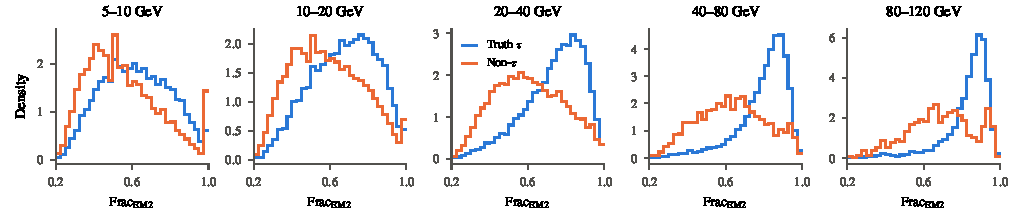
\includegraphics[width=\linewidth]{figures/fig_frac_conditioned.pdf}
  \caption{$\Frac$ for truth $\tau$ and non-$\tau$ objects in fixed $\ptTOB$ intervals (training split, normalised per class). The separation remains inside every interval and grows with energy, so the feature carries shape information beyond the energy scale.}
  \label{fig:frac_conditioned}
\end{figure}

% ============================================================================
\section{Feature Definitions}
\label{app:features}
% ============================================================================
Let $e$ be an event and $i$ an object in it. For layer $\ell\in\{\mathrm{EM0},\mathrm{EM1},\mathrm{EM2},\mathrm{EM3},\mathrm{HAD}\}$, $E_{\ell,ab}$ is the energy of tower $(a,b)$ of its $3\times3$ window. $E^{12}_{ab}$, $a,b\in\{0,\dots,11\}$, is the EM2 image. When a ratio has an exactly zero denominator, the implementation returns zero. Every entry below is a key of the feature registry and is selected through the experiment configuration.

\subsection{Input bundles}
\begin{itemize}
  \item \code{core\_tensors} (\CT): $x_i=\operatorname{vec}(E_{\mathrm{EM0}},E_{\mathrm{EM1}},E_{\mathrm{EM2}},E_{\mathrm{EM3}},E_{\mathrm{HAD}})\in\mathbb{R}^{45}$. Cell $9L+3r+c$ is layer $L$, row $r$, column $c$.
  \item \code{core\_physics} (\CP): $x_i=[\mathrm{BDT}_i,\ \ptTOBof{i},\ \eta_i-\eta_{\mathrm{lead}},\ \operatorname{wrap}(\phi_i-\phi_{\mathrm{lead}})]$, where ``lead'' is the highest-$\ptTOB$ object of the event and $\operatorname{wrap}$ maps an angle to $[-\pi,\pi)$.
  \item \code{em2\_all\_cells} (\EMtwo): $\operatorname{vec}(E^{12})\in\mathbb{R}^{144}$, reshaped to $1\times12\times12$ by the convolutional models.
  \item \code{tob\_pt\_only}: $x_i=\ptTOBof{i}$.
\end{itemize}

\subsection{Per-layer summaries}
\label{app:layer_summaries}
For every layer, with $S_\ell=\sum_{a,b}E_{\ell,ab}$ and $M_\ell=\max_{a,b}E_{\ell,ab}$,
\begin{equation}
  D_\ell = M_\ell-(S_\ell-M_\ell)=2M_\ell-S_\ell,\qquad
  Q_\ell=\sum_{a,b}\1\big[E_{\ell,ab}>0.1\,M_\ell\big].
\end{equation}
$S_\ell$ is the energy sum, $D_\ell$ the core dominance (the maximum cell minus its neighbours) and $Q_\ell$ the dynamic sparsity (the number of active cells). The 15 values $\{S_\ell,D_\ell,Q_\ell\}_\ell$ form the \SUM\ bundle. These definitions avoid cell-by-cell division, which was not available in the firmware specification of~\cite{kernan2026}.

\subsection{Full-granularity EM2 features}
\label{app:em2_features}
With $S^{12}=\sum_{a,b}E^{12}_{ab}$, $(a^\star,b^\star)=\arg\max_{a,b}E^{12}_{ab}$ and $d^2_{ab}=(a-a^\star)^2+(b-b^\star)^2$:
\begin{align}
  \Frac &= \frac{\max_{w\in\mathcal{W}_{3\times3}}\sum_{(a,b)\in w}E^{12}_{ab}}{S^{12}},
  &
  W_{\mathrm{norm}} &= \frac{\sum_{a,b}E^{12}_{ab}\,d^2_{ab}}{S^{12}},
\end{align}
the compactness (\code{em2\_best\_3x3\_fraction}) and the normalised shower width (\code{em2\_normalized\_width}). Further entries include the largest and second-largest cells, the squared distance between them (\code{em2\_maxdist}), the energy outside the best window divided by $\ptTOB$, and the energies and centre distances of the three strongest non-overlapping $3\times3$ windows. The registry also contains versions computed on the $3\times3$ EM2 core, and approximations that use subtraction instead of division. \code{em2\_3x3\_maxdist} is highly discrete. An early result that ranked it first is excluded: the earlier evaluation suffered from discrete-threshold defects, so that result was not a valid $0.5\%$ comparison. All results in this paper use the tie-aware calibration of \cref{app:calibration}.

\subsection{Event-level and object-geometry features}
With $r_1(e),r_2(e)$ the two leading objects:
\begin{equation}
  H_T^{\mathrm{TOB}}=\sum_{i\in e}\ptTOBof{i},\qquad
  \ptTOBof{r_2(e)},\qquad
  \Delta R_{12}=\sqrt{(\eta_{r_1}-\eta_{r_2})^2+\operatorname{wrap}(\phi_{r_1}-\phi_{r_2})^2} .
\end{equation}
These are computed once per event and copied to every object. For object-specific geometry, the partner $p(i)$ of object $i$ is the leading object other than $i$. The feature \code{object\_reference\_tob\_dr2} is $(\eta_i-\eta_{p(i)})^2+\operatorname{wrap}(\phi_i-\phi_{p(i)})^2$. The feature \code{object\_partner\_context} is $[\log(1+\ptTOBof{i}),\log(1+\ptTOBof{p(i)}),\pi-|\Delta\phi_{i,p}|,|\Delta\eta_{i,p}|]$, which keeps the partner energy, the azimuthal acoplanarity and the $\eta$ separation separate. In the distribution study, events with two or more $\tau$ objects have a much harder second-highest $\ptTOB$ and a larger $H_T^{\mathrm{TOB}}$ than events without a $\tau$. Their squared separation $\Delta R^2_{12}$ also peaks near $\pi^2$, the back-to-back topology. Background events populate the same region too, however. In our single-object tests, the event sum and the object-geometry features did not improve efficiency at $\FPRtarget$ over object-level inputs.

% ============================================================================
\section{Event-Level Calibration and Statistical Tools}
\label{app:calibration}
% ============================================================================

\subsection{Metrics, baseline and reporting protocol}
\label{app:metric_protocol}
The signal efficiency $\eff(\pT)$ is the fraction of truth-matched tau objects accepted at the calibrated threshold, rather than the fraction of signal events firing the trigger. It is reported globally over all test tau objects and in the true-$\pT$ bands $10$--$25$, $25$--$40$, $40$--$60$, $60$--$100$ and $100$--$120\GeV$. The event-level fake rate instead counts firing background events. The baseline accepts an object when $\ptTOB\geq C$ and uses the same two-object event decision as the network. Although this is a hard cut in reconstructed $\ptTOB$, its efficiency versus true $\pT$ turns on gradually because the reconstructed response is shifted and smeared; some high-true-$\pT$ objects still fall below the cut.

For the reported fixed-rate comparisons, the model and baseline thresholds are recalibrated on the same test background at the same target, and both achieved rates are reported. This measures discrimination at a common operating point; it does not test transfer of a frozen threshold. Performance using the validation-calibrated threshold is retained separately for that purpose. Test recalibration does not select features, losses, budgets, architectures or checkpoints. The design goal is non-inferiority above $\SI{25}{GeV}$, earlier saturation and gains across $25$--$100\GeV$, with some loss below $\SI{25}{GeV}$ acceptable. These are goals, not a claim that every reported model satisfies them. Accuracy, ROC-AUC and minimum BCE are not the primary selection criteria.

\subsection{Tie-aware threshold selection}
Let $\Bset$ be a set of $N$ background events. For the two-object trigger, the \emph{event trigger score} is $u_e=s_{e,(2)}$, the second-highest object score. An event with fewer than two objects can never fire. The procedure is:
\begin{enumerate}
  \item Let $v_1>v_2>\dots>v_m$ be the distinct values of $\{u_e\}$, and let $c_j=|\{e:u_e\geq v_j\}|$ be the cumulative counts (all events tied at a value are counted together).
  \item Let $k_{\max}=\lfloor\FPRtarget N\rfloor$. Return $t^\star=v_{j^\star}$ with $j^\star=\max\{j:c_j\leq k_{\max}\}$. If no such $j$ exists, return the next floating-point value above $v_1$, so that no event fires.
  \item Report the \emph{achieved} rate $\widehat{\FPR}=|\{e:u_e\geq t^\star\}|/N\leq\FPRtarget$.
\end{enumerate}
Because the search runs over distinct values, a group of tied scores is never split: all of its events pass or all fail. A threshold between two scores could claim a fake rate the deployed comparison $s\geq t$ cannot reproduce. Calibration and deployment use the same float64 comparison.

\subsection{Joint calibration of the OR classifier}
For a TOB budget $b$, the TOB cut $C_b$ is obtained by applying the procedure above to the second-highest $\ptTOB$ with target $b$. Given $C_b$, let $n_e=\sum_i\1[q_{e,i}\geq C_b]$ be the number of objects the TOB branch accepts in event $e$.
\begin{itemize}
  \item Events with $n_e\geq2$ fire regardless of the network. They form a fixed base count $N_0$.
  \item In an event with $n_e<2$, the network must accept $2-n_e$ of the remaining objects. The \emph{activation score} $u_e^{\mathrm{OR}}$ is the $(2-n_e)$-th highest network score among the objects the TOB branch did not accept. The event fires if and only if $u_e^{\mathrm{OR}}\geq t$.
\end{itemize}
The network threshold $t_b$ is the tie-aware threshold for the scores $\{u_e^{\mathrm{OR}}\}$ with the budget reduced by the base count, $k_{\max}-N_0$. This construction counts mixed events, in which one object passes each branch, exactly.

\subsection{Cross-fitting}
A threshold calibrated and evaluated on the same background events reports a fake rate of almost exactly $\FPRtarget$ by construction, and hides how well the threshold transfers to new events. Selection steps that compare many calibrated candidates therefore use two-fold cross-fitting. The events (never single objects) are split into two deterministic folds, stratified by class. The threshold is calibrated on fold A and all rates are measured on fold B, then the roles are swapped and the counts are pooled. This applies to the choice of the TOB budget, to checkpoint selection in constrained training, and to the dual updates on the training constraint subset. The plain target-FPR checkpoint rule (\cref{app:training}) calibrates and measures on the full validation set. After selection, one deployment threshold is calibrated on the complete validation set.

\subsection{Event-clustered paired uncertainty}
Guards compare a candidate classifier with a reference (the baseline or the pretrained model) on the \emph{same} truth $\tau$ objects of a region $r$. Let $d_i=\1[\text{candidate accepts }i]-\1[\text{reference accepts }i]$, let $n$ be the number of objects, $\hat\Delta_r=\frac1n\sum_i d_i$, and $D_e=\sum_{i\in e}d_i$ with $n_e$ objects in event $e$. Objects of one event are correlated, so the standard error is clustered by event ($G$ events):
\begin{equation}
  \hat\sigma_r^2=\frac{G}{G-1}\,\frac{\sum_e\big(D_e-\hat\Delta_r n_e\big)^2}{n^2},
  \qquad L_r=\hat\Delta_r-z\,\hat\sigma_r .
\end{equation}
$L_r$ is a one-sided lower confidence bound. The OR budget search uses $z=1$, and constrained-training selection uses $z=z_{0.95}$.

\subsection{Confidence-safe deployment target}
Let $U(k,N)$ be the exact one-sided Clopper--Pearson upper bound~\cite{clopper1934} on a binomial rate with $k$ firing events out of $N$, $U(k,N)=\mathrm{Beta}^{-1}(1-\alpha;\,k+1,\,N-k)$. The confidence-safe target is $k^\star/N$, where $k^\star$ is the largest $k\leq\lfloor\FPRtarget N\rfloor$ with $U(k,N)\leq\FPRtarget$. The deployed threshold is calibrated to this lower empirical rate. With the validation statistics available, the one-sided $95\%$ target corresponds to an empirical fake rate of about $0.42\%$.

% ============================================================================
\section{The TOB--NN OR Classifier}
\label{app:or}
% ============================================================================

\subsection{From a mixture of experts to a logical OR}
With plain BCE and $\ptTOB$ among the inputs, the learned turn-on curve often resembled the TOB baseline from below. The network learned most of the energy dependence but not enough shape information to beat the baseline at high energy. Our first remedy was a two-expert model: an energy expert with inputs such as $\ptTOB$, and a shape expert with $\Frac$, widths and angular variables. The two were combined as $s_{\mathrm{mix}}=\alpha s_{\mathrm{energy}}+(1-\alpha)s_{\mathrm{shape}}$, with $\alpha$ and the threshold chosen on validation. Preliminary runs gave no meaningful gain, and the energy expert only relearned a rule that the eFEX already implements exactly. The OR classifier~\eqref{eq:or} keeps this rule deterministic and gives the network the complementary task.

\subsection{Joint calibration}
Given a TOB budget $b$, the comparator threshold $C_b$ is set so that the TOB branch alone fires in at most a fraction $b$ of background events. The NN threshold $t_b$ is then calibrated so that the complete OR fires in at most $\FPRtarget$. Both steps operate on event decisions: an event containing one TOB-accepted object and one distinct NN-accepted object must count as accepted, even when neither branch alone would fire. The budget is selected separately for each model on validation, not assigned during training.

\subsection{Per-epoch selection procedure}
At the end of every training epoch:
\begin{enumerate}
  \item the network is trained with (weighted) BCE; the OR rule does not enter the gradient;
  \item validation scores are predicted;
  \item for every candidate $b\in\mathcal{B}=\{0,0.0005,\dots,0.005\}$, the pair $(C_b,t_b)$ is calibrated with two-fold event cross-fitting inside the validation set (\cref{app:calibration});
  \item candidates that exceed the $0.5\%$ event fake rate or violate a protection guard are discarded;
  \item the feasible candidate with the largest objective $J(b)$~\eqref{eq:or_objective} is selected; when two objectives differ by at most $0.002$, the one with the safer worst-window margin is preferred;
  \item epochs are compared with the same objective.
\end{enumerate}
The minimum-BCE checkpoint is kept as a reference. No budget, threshold or epoch is chosen on test data. The procedure is repeated independently for every feature set, seed and checkpoint, because the score distribution of the network and its overlap with the TOB branch change with the inputs.

\subsection{Objective}
The target is the mean efficiency advantage over the region of interest,
\begin{equation}
  J_{\mathrm{cont}}(b)=\frac{1}{100-25}\int_{25}^{100}\big[\eff_{\mathrm{OR}}(p;b)-\effTOB(p)\big]\,dp .
\end{equation}
It is estimated over $5\GeV$ windows spanning $25$--$100\GeV$:
\begin{equation}
  J(b)=|\Kset|^{-1}\sum_{k\in\Kset}\big[\hat\eff_{\mathrm{OR},k}(b)-\hat\eff^{\mathrm{TOB}}_k\big].
  \label{eq:or_objective}
\end{equation} Equal window weights state the physics preference directly: a gain in a sparsely populated high-energy window counts as much as one near the threshold.

\subsection{Protection guards}
\begin{description}[leftmargin=0pt,itemsep=2pt]
  \item[Per window.] The original rule required $\hat\Delta_k\geq-0.005$ in every $5\GeV$ window up to $\SI{120}{GeV}$. It proved too sensitive to fluctuations: saturated validation windows contain only $90$--$250$ truth $\tau$ objects, so one object moves the efficiency by $0.4$--$1.1$ points, and a candidate could be accepted or rejected because of a single object.
  \item[Pooled saturation.] The $5\GeV$ guards are kept below $\SI{60}{GeV}$, and all guards above are replaced by one pooled region with $\hat\Delta_{60:120}\geq-0.005$. Pooling increases the sample, but a local deficit can be averaged away.
  \item[Multiscale saturation.] The fine guards are kept below $\SI{60}{GeV}$. The saturation range is tested on the overlapping regions $[60,90)$, $[70,100)$, $[80,110)$, $[90,120)$ and the full $[60,120)$, each with the event-clustered lower bound $L_r=\hat\Delta_r-z\hat\sigma_r\geq-\delta_{\mathrm{phys}}$ ($z=1$, $\delta_{\mathrm{phys}}=0.005$). The overlapping regions detect a persistent local loss that pooling would hide, and they are more stable than $5\GeV$ windows. A tolerance of $\delta_{\mathrm{phys}}=0$ was needlessly strict, because it demanded a statistically positive gain even where both classifiers are already close to full efficiency.
\end{description}

\subsection{Interpreting the selected budget}
A small $b^\star$ leaves more of the background budget to decisions introduced by the network, and usually indicates a larger independent contribution from the NN. A large $b^\star$ indicates stronger reliance on the comparator. This reading is useful but not absolute, because $b^\star$ also depends on score calibration, seed fluctuations and the overlap of the two branches. The budget changes the final decision rule, whereas signal weighting (\cref{app:weighting}) changes the learned score. The two are separate mechanisms and were studied separately.

% ============================================================================
\section{Energy-Weighted BCE}
\label{app:weighting}
% ============================================================================
For an object with label $y_i$, score $s_i$ and weight $w_i$,
\begin{equation}
  \mathcal{L}_{w}=-\frac1N\sum_{i=1}^{N}w_i\big[y_i\log s_i+(1-y_i)\log(1-s_i)\big].
\end{equation}
Background objects always keep $w_i=1$. They have no meaningful true $\tau$ momentum, and reweighting them would distort the rare background tail that sets the $0.5\%$ event fake rate. Signal weights are built from a raw profile $r(t)$ of the true momentum $t$ (in GeV) and normalised on the \emph{training} signal only:
\begin{equation}
  w_i=\frac{r(t_i)}{\frac{1}{N_S}\sum_{j\in\Sset_{\mathrm{train}}}r(t_j)},\qquad y_i=1 .
\end{equation}
The mean training signal weight is therefore one, so a profile redistributes the signal gradient across energy without changing the overall signal--background balance. A profile fitted on training data is reused unchanged on validation data. Truth momentum is used only to build weights, never as an input.

\subsection{Turn-on emphasis (\texorpdfstring{$\alpha$}{alpha} profile)}
The first hypothesis was that the TOB branch already protects the plateau, so the network should concentrate on the turn-on:
\begin{equation}
  r_\alpha(t)=\begin{cases}1,& t<25,\\ 1+\alpha,& 25\leq t<40,\\ 1+\alpha/2,& 40\leq t<80,\\ 1,& t\geq80,\end{cases}
  \qquad \alpha\in\{0,1,2,4\}.
\end{equation}
$\alpha=0$ is exactly plain BCE and serves as a control. Every $\alpha$ is a separate training run with $\alpha$ fixed throughout.

\subsection{Inverse-frequency profile}
The range $25$--$100\GeV$ is divided into $5\GeV$ bins. With $n_k$ training-signal objects in populated bin $k\in\Kset_+$,
\begin{equation}
  \bar n=\frac{1}{|\Kset_+|}\sum_{k\in\Kset_+}n_k,\qquad r_k=\operatorname{clip}\Big(\frac{\bar n}{n_k},\,0.2,\,5\Big),
\end{equation}
and $r=1$ outside the range. Without clipping, $n_kr_k\approx\bar n$: every bin contributes the same total signal weight. The clipping keeps a nearly empty bin from producing an unstable gradient. For seed~42 the fitted weights are about $0.39$ at $25$--$30\GeV$, $0.57$ at $35$--$40$, $0.96$ at $50$--$55$, $1.36$ at $60$--$65$, $2.06$ at $75$--$80$ and $3.28$ at $95$--$100\GeV$.

\subsection{Power-law profile}
Above $\approx\SI{25}{GeV}$ the training $\tau$ spectrum is well described by $f_S(t)\approx c/t^2$. The unweighted signal contribution of a narrow interval $[t_0,t_0+dt]$ to BCE is then
\begin{equation}
  d\mathcal{L}_S(t_0)\propto\frac{1}{t_0^2}\,\E\big[\ell_{\mathrm{BCE}}\mid t_0\big]\,dt .
\end{equation}
A $25$--$30\GeV$ bin contains about eight times as many training taus as a $95$--$100\GeV$ bin. Even when the average loss per object is similar at all energies, soft $\tau$ objects dominate the gradient because there are many more of them. Plain BCE therefore already favours the dense, low-energy part of the spectrum. For a one-parameter control over this effect, we clamp $\tilde t_i=\min(200,\max(10,t_i))$ and set $r_p(t_i)=\tilde t_i^{-p}$. Away from the clamp,
\begin{equation}
  f_S(t)\,w_p(t)\propto t^{-(2+p)} .
\end{equation}
\begin{itemize}
  \item $p=0$: plain BCE.
  \item $p>0$: relatively more weight on low-$\pT$ $\tau$ objects.
  \item $p<0$: relatively more weight on high-$\pT$ $\tau$ objects.
  \item $p=-1$: equal weighted signal counts per logarithmic interval, since $t^{-1}dt=d\log t$.
  \item Inverse frequency: for equal-width bins and $f_S\propto t^{-2}$, it behaves roughly like a clipped $t^{2}$ weight, i.e. qualitatively $p\approx-2$.
\end{itemize}
IF is not the power-law profile at $p=-1$ (or exactly at $p=-2$): it uses empirical counts, different clipping and unit raw weights outside $25$--$100\GeV$. The clamp keeps very small or very large momenta from producing extreme weights. The screen covered $p\in\{-1.9,-1.6,-1.3,-1,-0.6,-0.3,0.3,0.6,1\}$, together with plain BCE and inverse frequency. The negative side was extended after the first screen favoured more weight on high-energy $\tau$ objects.

\subsection{Why emphasising energetic taus can help soft ones}
We propose a mechanism, not a proof. Energetic $\tau$ showers have a higher signal-to-noise ratio, more stable shape measurements and less overlap with background, so they are cleaner examples of the class. A representation learned from them can transfer to weaker, low-energy showers. Strongly up-weighting soft objects instead emphasises noisy or intrinsically ambiguous examples, raises the gradient variance and moves the decision boundary without teaching a more general $\tau$ signature. The mechanism is consistent with the smaller TOB budgets selected under inverse-frequency weighting (\cref{app:or}). No weight profile is optimal in general: the best profile depends on the features, the model capacity, the optimisation and the class overlap.

% ============================================================================
\section{The Constrained Trigger Objective}
\label{app:constrained}
% ============================================================================

\subsection{Problem}
Let $s_i=f_\theta(x_i)$. Under the NN-only classifier an object passes when $s_i\geq t$. Under the OR classifier it passes when $(\ptTOBof{i}\geq C)\vee(s_i\geq t)$. The same event rule~\eqref{eq:event_decision} applies in both cases. One list of energy regions should not serve two purposes: improvement is wanted where there is room for it, while protection is needed everywhere. The objective regions and weights are
\begin{equation}
  \Kset_J=\{[25,32),[32,40),[40,60)\}\GeV,\qquad w=(0.35,0.35,0.30),\quad\textstyle\sum_k w_k=1,
\end{equation}
and the constraint regions are $\Kset_C=\Kset_J\cup\{[60,120)\}$. The turn-on window is split at $\SI{32}{GeV}$ because the measured advantage changes strongly inside $[25,40)$. The saturated region is left out of the objective: its attainable gain is bounded by $1-\effTOB_{60:120}\approx0.03$, and its measured advantage is comparable to its statistical uncertainty. The weights encode a fixed scientific preference and are not learned, because an optimiser allowed to choose them would put all weight on the easiest region. Each constraint region carries the floor
\begin{equation}
  r_k=\min\Big[1,\;\max\big(\effTOB_k+m_k,\;\eff_k^{(0)}-\rho_k\big)\Big],
  \label{eq:floor}
\end{equation}
where $m_k$ is the required advantage over the baseline, $\eff_k^{(0)}$ is the efficiency of the frozen pretrained network, and $\rho_k$ is the largest loss allowed relative to it. We use $m=(0.0025,0.0025,0.0025,0)$ and $\rho=(0.0025,0.0025,0.0025,0.005)$. The second term is needed because fine-tuning starts from a strong model: a guard that protects only the baseline allowed the network to give up part of an advantage it already had. The complete problem is
\begin{equation}
  \max_\theta\;J(\theta)=\sum_{k\in\Kset_J}w_k\big[\eff_k(\theta)-\effTOB_k\big]
  \quad\text{s.t.}\quad\FPRev(\theta)\leq0.005,\quad\eff_k(\theta)\geq r_k\;\;\forall k\in\Kset_C .
\end{equation}

\subsection{Differentiable surrogate}
The hard threshold and the ``at least two'' count have zero gradient almost everywhere. The network update therefore uses smooth surrogates, while every constraint measurement uses the exact hard decisions.
The construction replaces an object step by a temperature-controlled sigmoid and the event count by the probability of at least two successes under the surrogate's independent Bernoulli decisions. This is a differentiable device, not an assumption that physical objects within an event are independent. As $T\to0$, it approaches the hard decision away from threshold ties.
\begin{description}[leftmargin=0pt,itemsep=2pt]
  \item[Soft object decision.] $q_i=\sigmoid\big((z_i-t_{\mathrm{proxy}})/T\big)$, where $z_i$ is the pre-sigmoid score (logit) of object $i$. For the OR classifier the comparator stays hard: $q_i^{\mathrm{OR}}=h_i+(1-h_i)q_i$ with $h_i=\1[\ptTOBof{i}\geq C]$.
  \item[Rank-calibrated proxy threshold.] In every batch, $t_{\mathrm{proxy}}$ is recomputed as the empirical background quantile that matches the $0.5\%$ event target, taken from the ranked second-highest object logits of the background events in the batch. A common shift of all scores then moves the threshold by the same amount, so the score-inflation direction carries no gradient.
  \item[Temperature annealing.] The gradient of $q_i$ is proportional to $q_i(1-q_i)/T$ and becomes negligible for $|z_i-t_{\mathrm{proxy}}|\gtrsim3T$. A small temperature $T$ gives a faithful surrogate that sees only a narrow band around the boundary. A large $T$ reaches distant objects but optimises a blurred trigger. $T$ therefore follows a cosine schedule from $0.10$ to $0.02$.
  \item[Event surrogate.] The probability that at least two objects pass is the Poisson-binomial tail
  \begin{equation}
    \tilde P_e^{(2)}=1-\prod_{i\in e}(1-q_i)-\sum_{i\in e}q_i\prod_{j\in e,\,j\neq i}(1-q_j).
    \label{eq:surrogates}
  \end{equation}
  With $\Bset$ the background events and $\Sset_k$ the truth $\tau$ objects of region $k$, $\widetilde{\FPR}=|\Bset|^{-1}\sum_{e\in\Bset}\tilde P_e^{(2)}$ and $\tilde\eff_k=|\Sset_k|^{-1}\sum_{i\in\Sset_k}q_i$. These quantities are used only for optimisation and never to certify a constraint.
\end{description}

\paragraph{Why recalibration matters.}
With a frozen proxy threshold, the optimiser could increase every score through the output bias, improving the soft objective without improving the deployed ranking; the fake rate at that frozen threshold grew several-fold. Recomputing the proxy threshold from background ranks makes it move with a common score shift and removes this artificial gain. This addresses score translation; it does not imply that a fixed-temperature sigmoid surrogate is invariant to every monotone score transformation. Annealing then trades broad early gradient coverage for a sharper late approximation.

\subsection{Primal--dual training}
The Lagrangian is
\begin{equation}
  \mathcal{L}(\theta,\lambda)=-\tilde J(\theta)+\lambda_{\mathrm{FPR}}\frac{\widetilde{\FPR}(\theta)-0.005}{0.005}+\sum_{k\in\Kset_C}\lambda_k\big(r_k-\tilde\eff_k(\theta)\big),
\end{equation}
where $\tilde J$ replaces each hard efficiency by its surrogate. The fake-rate violation is expressed relative to its target so that the fake-rate and region terms have comparable scales. Without this normalisation, a one-per-mille excess in fake rate would be numerically invisible next to an efficiency deficit of the same physical importance. The two updates alternate. The network parameters take Adam steps on $\mathcal{L}$. The multipliers follow projected dual ascent on \emph{hard} violations $g_j$,
\begin{equation}
  \lambda_j\leftarrow\big[\lambda_j+\eta_j\,g_j\big]_{[0,\lambda_{\max}]},\qquad\lambda_{\max}=25,\quad\eta_{\mathrm{FPR}}=1,\quad\eta_k=50 .
\end{equation}
All multipliers start at zero and become active only after a measured violation. The region rates are larger because region violations are numerically small: they correspond to a handful of signal objects. The hard violations are measured once per epoch on a held-out \emph{constraint subset} of the training events, with two-fold cross-fitting. This keeps optimistic in-sample calibration from driving the multipliers: in earlier stages the in-sample measurement reported comfortable margins while the validation margins were already negative, and every $\lambda_k$ stayed at zero throughout training. The division of labour is strict: differentiable quantities provide gradients, and exact deployable decisions determine whether a constraint is satisfied.

\subsection{Protocol and leakage protection}
Constrained training is a fine-tuning stage. It starts from the best weighted-BCE checkpoint of the same input representation and runs for $20$ epochs at learning rate $10^{-4}$, with batches of $2048$ complete events. The training events are split into two disjoint, stratified subsets: a primal subset ($70\%$) for the network update and a constraint subset ($30\%$) used only for the dual update. Complete events stay together, because the event fake rate cannot be estimated from shuffled objects. Checkpoint selection uses validation cross-fitting (\cref{app:calibration}). The held-out validation fake rate measured this way is typically $0.35$--$0.40\%$, while the in-sample value is $0.499\%$. After the best epoch is chosen, one deployment threshold is calibrated on the full validation set with the confidence-safe target. The test set is never used for training, calibration or selection.

\subsection{Uncertainty-aware feasibility}
Feasibility based on point estimates was fragile in both directions. A checkpoint could be accepted because a window of 90 objects fluctuated upward, or rejected because it fluctuated downward. Every constraint is therefore evaluated with its event-clustered lower bound $L_r$ (\cref{app:calibration}). The first fully certified rule required $L_r\geq m_k$ in every region and a certified fake-rate bound below target. It was too strict: certifying a $0.5\%$ rate at $95\%$ confidence requires operating near $0.42\%$, and certifying a non-negative advantage in the saturated region requires an observed advantage of about $+0.8$ points where the true value is compatible with zero. Even the initial model was infeasible, and two of three seeds returned their initialisation. The corrected rule keeps the uncertainty machinery but
(i)~applies the fake-rate test to the measured cross-fitted rate and records the Clopper--Pearson bound as a diagnostic (the budget itself is protected by the confidence-safe deployment target), and
(ii)~includes the tolerance in the certified guards, $L_r\geq m_k-\delta_{\mathrm{phys}}$ with $\delta_{\mathrm{phys}}=0.005$, so a saturated region must be statistically compatible with non-inferiority rather than certifiably superior.
Among feasible epochs, the one with the largest cross-fitted hard objective is selected. If no epoch is feasible, the one with the smallest certified violation is kept.

\subsection{Applying the loss to other inputs and to the CNNs}
The objective, the constraints, the surrogates and the dual updates act only on network scores and measured efficiencies, and no term refers to the input variables. A different input representation is therefore a configuration change, not a code change. Three surrounding components are matched to the representation and are prepared for each one:
\begin{itemize}
  \item \textbf{Initialisation and reference guard.} Fine-tuning starts from the best weighted-BCE model of the \emph{same} inputs: inverse frequency for \CT\ and \SUM+\Ffeat, and $p=-1$ for \CP+\CT\ and \CT+\Ffeat. The reference floor~\eqref{eq:floor} is defined relative to this starting point, so a checkpoint trained on other inputs cannot be reused.
  \item \textbf{Temperature scale.} $T$ acts on the score scale, and different inputs produce score distributions of different width near the threshold. The fraction of objects inside the effective gradient band $|z_i-t_{\mathrm{proxy}}|\lesssim3T$ is recorded per region before training. The annealing endpoints are changed only if this coverage differs strongly from the reference.
  \item \textbf{What transfers unchanged.} Across the MLP inputs, the regions, weights and tolerances ($m_k$, $\rho_k$, $\delta_{\mathrm{phys}}$) are physics choices in efficiency units. The dual rates and the fake-rate normalisation act on rate scales. The cross-fitting, the confidence-safe calibration and the selection protocol are independent of the inputs.
\end{itemize}
The same recipe is used for the convolutional models, where ``FT'' denotes a constrained fine-tune of an IF or BCE model (\cref{tab:naming}). Their weak end was saturation rather than the turn-on, so for them the objective also rewards $[60,100)\GeV$, with weights $w=(0.30,0.30,0.25,0.15)$, and the saturated region is guarded as two regions, $[60,100)$ and $[100,120)\GeV$, each allowed at most $0.5$ points below the starting model. This is the only change of regions or weights between input representations.

\subsection{Discarded variants}
\begin{description}[leftmargin=0pt,itemsep=2pt]
  \item[Frozen proxy threshold with a counterweight.] Keeping $t_{\mathrm{proxy}}$ fixed and relying on $\lambda_{\mathrm{FPR}}$ (initialised by balancing gradient norms) to suppress score inflation only moved the equilibrium: each seed settled at a different inflation level. The rank-calibrated threshold removes the direction from the loss itself.
  \item[Tail-ranking objective.] A pairwise logistic loss compared truth-$\tau$ logits with the second-highest logits of the top $5\%$ of background events, selected by rank. It is shift invariant and gives full gradient to signal far below the boundary. However, it raised the low-energy gain faster than the saturation constraints could respond, and checkpoint selection fell back to early epochs.
  \item[Hard-negative memory bank.] A buffer of median-centred background offsets from earlier batches was meant to enlarge the ranking tail. The stale offsets no longer matched the current network, and all seeds selected their initialisation.
\end{description}

\subsection{Requirements for a trigger loss}
\label{app:loss_requirements}
These requirements emerged from failed variants as well as successful fine-tuning. Weighted BCE captured much of the available improvement; the custom objective chiefly made energy-dependent trade-offs explicit. The lessons concern the complete loss, calibration and selection procedure, not a claim that one surrogate is universally optimal.
\begin{enumerate}[label=(\arabic*),itemsep=3pt]
  \item \textbf{Respect the calibrated ranking.}
  After threshold recalibration, a common strictly increasing transformation of the scores preserves their ranking and hence the hard decision at a fixed rate, apart from numerical or tie effects. A surrogate should not reward changes that merely move all scores together. With a frozen proxy threshold, output-bias inflation increased the training fake rate from $0.5\%$ to above $3\%$ without improving separation. A minimal diagnostic is to add a constant to every logit and verify that the objective does not improve. Recomputing the background-quantile threshold removes this translation shortcut; it does not make a fixed-temperature sigmoid invariant to arbitrary monotone transformations.

  \item \textbf{Make regional trade-offs explicit.}
  Equal object weights are not equal energy-region weights: the falling spectrum gives abundant soft taus more influence. A region absent from both reward and protection can pay for gains elsewhere. In the \SUM+\Ffeat\ fine-tune, improvements at $32$--$60\GeV$ accompanied a $0.69$-point loss at $10$--$25\GeV$, which had neither role. Every scientifically relevant region therefore needs an explicit reward, floor or deliberately accepted trade-off. Adaptive constraint multipliers cannot protect a region omitted from the formulation.

  \item \textbf{Inspect gradient coverage, not just the loss value.}
  A narrow sigmoid surrogate can be accurate near the threshold yet give almost no gradient to missed taus far below it. In one examined setting, their gradient magnitude was about $1/4600$ of that at the boundary. Conversely, the tail-ranking variant reached distant signal but changed the efficiency profile faster than the protection mechanism could react. Inspect gradient magnitude against score and energy, including missed signal; temperature annealing balances early reach against late decision fidelity.

  \item \textbf{Optimise softly, assess hard decisions out of sample.}
  Differentiability is a training device, not evidence of constraint satisfaction. Threshold calibration and violation measurement must use separate event subsets through cross-fitting, and measurements must use the exact two-object trigger. Earlier in-sample checks reported safe regional margins while held-out margins were negative, leaving all regional multipliers inactive. Held-out constraint events restored meaningful feedback; validation remained separate for checkpoint selection.

  \item \textbf{Match tolerances to statistical resolution.}
  Sparse windows cannot support arbitrarily fine protection thresholds: one accepted tau among $90$--$250$ objects changes efficiency by roughly $0.4$--$1.1$ percentage points. The first fully certified rule rejected even the initial model; pooled or multiscale guards and uncertainty-aware tolerances made selection usable. Compute uncertainty at the level of the claim, preserving event clustering and paired comparisons where appropriate. A small global gain across seeds and an equally sized fluctuation in one sparse bin are not equally strong evidence.
\end{enumerate}

\subsection{Detailed explanation from the main methodology}
In the original MLP formulation, the regions to improve, $\Kset_J=\{[25,32),[32,40),[40,60)\}\GeV$, are kept separate from the regions to protect, $\Kset_C=\Kset_J\cup\{[60,120)\}$. The saturated region is protected but not rewarded, because there is almost no room for gain there and its measurement is dominated by noise. The CNN extension also rewards $60$--$100\GeV$ and splits the saturation guards (\cref{app:constrained}). We train on the Lagrangian of~\eqref{eq:constrained}:
\begin{equation}
  \mathcal{L}(\theta,\lambda)=
  -\underbrace{\sum_{k\in\Kset_J}w_k\big[\tilde\eff_k(\theta)-\effTOB_k\big]}_{\text{reward: turn-on gain}}
  +\lambda_{\mathrm{FPR}}\underbrace{\frac{\widetilde{\FPR}(\theta)-\FPRtarget}{\FPRtarget}}_{\text{fake-rate violation}}
  +\sum_{k\in\Kset_C}\lambda_k\underbrace{\big(r_k-\tilde\eff_k(\theta)\big)}_{\text{deficit in region }k}.
  \label{eq:lagrangian}
\end{equation}
\begin{itemize}
  \item The \emph{reward} is the efficiency gain over the baseline in the turn-on regions. For the MLP, its fixed weights $w=(0.35,0.35,0.30)$ state our physics preference. They are not learned, because an optimiser allowed to choose them would put all the weight on the easiest region.
  \item The \emph{fake-rate term} measures the violation relative to the $0.5\%$ target. Without this normalisation, an excess of one per mille would be numerically invisible next to an efficiency deficit of the same physical importance.
  \item Each \emph{region term} compares the efficiency with a floor $r_k$. The floor requires a small margin over the baseline and allows at most a small loss relative to the pretrained starting model.
  \item The multipliers $\lambda\geq0$ act as adaptive prices. The network parameters $\theta$ descend on $\mathcal{L}$ with Adam. Each price starts at zero, rises by projected dual ascent only while its constraint is \emph{measured} to be violated by the exact deployed rule, and falls back when it is satisfied~\cite{cotter2019proxy}. A fixed weight profile is the special case in which these prices are guessed in advance.
\end{itemize}
The hard threshold and two-object event rule have no useful gradient, so training uses smooth approximations while constraint checks use exact decisions. Four choices stabilise this separation:
\begin{enumerate}[label=(\roman*),itemsep=1pt,topsep=2pt]
  \item \textbf{Recalibrate the proxy threshold.} A batch-wise background quantile prevents uniformly raising all scores from appearing to improve classification.
  \item \textbf{Anneal the temperature.} A broad early sigmoid reaches more objects; cooling from $0.10$ to $0.02$ sharpens it towards the hard decision.
  \item \textbf{Measure violations out of sample.} Cross-fitting on a held-out $30\%$ of training events prevents optimistic in-sample estimates from suppressing the dual updates.
  \item \textbf{Start from a trained model and respect uncertainty.} Fine-tune a BCE-based checkpoint, allow statistically meaningful tolerances and calibrate deployment conservatively.
\end{enumerate}
\Cref{app:constrained} gives the equations, feasibility rules and discarded variants.

% ============================================================================
\section{Model Names and Architectures}
\label{app:arch}
% ============================================================================

\subsection{How to read a model name}
\label{app:naming}
A model name lists its inputs and architecture, then its training objective and classifier (\cref{tab:naming}). Two examples:
\begin{itemize}
  \item ``E1+V4+\Ffeat, IF'': an EM2 branch of type E1, a core-tensor backbone of type V4 and the $\Frac$ scalar, joined in the dense head and trained with inverse-frequency weighted BCE. The classifier is NN-only (the default).
  \item ``MLP, \CT+\Ffeat, FT'': the $[32,16]$ MLP on the 45 core cells plus $\Frac$, pretrained with weighted BCE and then fine-tuned with the constrained objective.
\end{itemize}
A V-backbone implicitly consumes \CT; an E-branch implicitly consumes the fine EM2 image. A suffix $+\Ffeat$ adds the engineered scalar, not another image. Flat \CT\ or \SUM\ bypasses convolution and enters the head directly. Unless OR is specified, the classifier is NN-only. Thus E3+V2+\Ffeat, FT means EM2 branch E3, core backbone V2 and Fraction, first trained with IF and then constrained-fine-tuned; it does not mean a power-law run.

\begin{table}[h]
  \centering
  \caption{Naming key for inputs, architectures, objectives and classifiers.}
  \label{tab:naming}
  \small
  \begin{tabularx}{\linewidth}{@{}lX@{}}
    \toprule
    Name & Meaning \\
    \midrule
    \multicolumn{2}{@{}l}{\emph{Inputs}} \\
    \CT & the 45 raw cell energies of the $5\times3\times3$ core tensor (\cref{app:features}) \\
    \SUM & 15 per-layer summaries: energy sum, core dominance and sparsity of each of the five layers \\
    \CP & ``core physics'': BDT score, $\ptTOB$, and $\eta,\phi$ relative to the leading TOB \\
    \Ffeat & the EM2 compactness $\Frac$ (\cref{eq:frac}) \\
    \EMtwo & the $12\times12$ EM2 image; read only by an E-branch \\
    flat \CT\ / \SUM & the cells or summaries passed directly to the dense head, without convolution \\
    \midrule
    \multicolumn{2}{@{}l}{\emph{Architectures}} \\
    MLP & fully connected network $d\to32\to16\to1$ \\
    V1 & core-tensor layer mixing: $1\times1$ convolution across five input layers, 12 filters \\
    V2 & core-tensor spatial processing: $2\times2$ convolution across five layers, 12 filters \\
    V3 & serial core backbone: V1 followed by a $2\times2$ convolution on its feature maps \\
    V4 & parallel core backbone: V1 and V2 outputs concatenated (\cref{app:vbackbones}) \\
    E1 & EM2: $3\times3$ convolution, 4 filters, then $2\times2$ max pooling \\
    E2 & EM2: $3\times3$ convolution, 8 filters, pooling, then a second $3\times3$ convolution \\
    E3 & EM2: as E2, but stride 2 replaces first-stage pooling (\cref{app:ebranches}) \\
    E$x$+V$y$ & dual-branch model: E-branch and V-backbone concatenated in one head \\
    E$x$ + flat \CT & EM2-only model: an E-branch plus plain core-cell scalars (\cref{app:em2only}) \\
    \midrule
    \multicolumn{2}{@{}l}{\emph{Training objective}} \\
    BCE & plain binary cross-entropy \\
    IF & inverse-frequency BCE: signal weights from empirical training-bin counts, with clipping (\cref{app:weighting}) \\
    $p$ & power-law BCE: weights proportional to clamped $t^{-p}$; $p<0$ emphasises energetic signal. Not the IF formula \\
    FT & constrained fine-tuning of a pretrained model; an unqualified CNN FT starts from IF \\
    BCE+FT / $p{=}-1$+FT & FT after plain BCE / power-law BCE with $p=-1$, respectively \\
    rank control & earlier rank-calibrated soft-objective FT control, not the pairwise tail-ranking variant \\
    \midrule
    \multicolumn{2}{@{}l}{\emph{Classifier}} \\
    NN-only & default: an object is accepted when $s_{e,i}\geq t$ \\
    OR & TOB--NN OR classifier~\eqref{eq:or} \\
    \bottomrule
  \end{tabularx}
\end{table}

\subsection{Common interface}
All models share one interface: \code{forward} returns a probability and \code{forward\_logits} returns the pre-sigmoid score. Training, calibration and constrained fine-tuning therefore treat every model in the same way. A configuration without a \code{model} block reproduces the MLP exactly. Setting \code{model.name=tensor\_cnn} builds a convolutional model from a list of branches. Each branch names a registry feature and a shape, and folds that feature's columns back into a (channels, height, width) image in the same order as the registry. Kernel sizes, channel counts, strides, pooling, extra branches and skip connections are all configuration fields, so a new architecture is a new configuration rather than new code.

\subsection{MLP}
The MLP is $d\to32\to16\to1$ with ReLU activations and a sigmoid output, and has $32d+577$ parameters. For example, it has $2{,}049$ parameters on \CT+\Ffeat\ ($d=46$), $2{,}145$ on \CP+\CT\ and $1{,}089$ on \SUM+\Ffeat. \citet{kernan2026} also swept the hidden layers $[48]$, $[32,32]$, $[64,32]$, $[32,16,8]$, $[64,32,16]$, $[64,32,16,8]$, $[64,32,16,8,8]$ and $[512,256,128,64,32]$ over seven feature sets, and found no systematic change in the turn-on curve. The largest network was the weakest on the largest input.

\subsection{Core-tensor backbones V1--V4}
\label{app:vbackbones}
The core tensor is a stack of five $3\times3$ images, one per calorimeter layer (\cref{fig:cnn_blocks}a). A convolution slides one small set of weights, the \emph{kernel}, over the image and applies the same weights at every position. This builds in two assumptions an MLP must learn from data: nearby cells are related, and the same pattern means the same thing wherever it appears. On a $3\times3$ grid a $3\times3$ kernel fits in only one position, so it is no different from a dense layer. Only two kernel shapes give real weight sharing:
\begin{itemize}
  \item \textbf{V1, layer mixing ($1\times1\times5$).} At each of the nine cells, the kernel reads the five energies of that cell, one per layer from EM0 to HAD, and forms a weighted sum. Twelve such filters give twelve numbers per cell. Each filter is a learned description of the \emph{longitudinal profile}, i.e.\ how the energy is shared between the layers, and the same filter is applied at every cell. The output is $12\times3\times3=108$ values from $72$ weights.
  \item \textbf{V2, spatial ($2\times2\times5$).} The kernel reads a $2\times2$ block of cells across all five layers ($20$ energies) and fits at four positions. Its twelve filters learn local spatial patterns, such as ``energy in the centre but not in its neighbour'', in all layers at once. The output is $12\times2\times2=48$ values from $252$ weights.
  \item \textbf{V3, serial.} V1 first converts each cell into twelve profile values. A $2\times2$ convolution over these twelve channels then looks for spatial patterns in the learned profiles. The output is $48$ values.
  \item \textbf{V4, parallel.} V1 and V2 run side by side on the same input, and their outputs are concatenated ($108+48=156$ values). Each mechanism can specialise without passing through the other.
\end{itemize}
The window is centred on the TOB seed, so the absolute position of a pattern is informative: a large central cell means something different from a large corner cell. We therefore never apply global pooling; the feature maps are flattened and fed to the dense head together with any scalar inputs.

\subsection{EM2 branches E1--E3}
\label{app:ebranches}
The $12\times12$ EM2 image is large enough for standard convolution blocks (\cref{fig:cnn_blocks}b).
\begin{itemize}
  \item \textbf{E1, single block.} A $3\times3$ kernel slides over the image with stride~1, which gives $10\times10=100$ positions. Four filters with $9$ weights and a bias each ($40$ parameters) act as four learned templates, such as an isolated peak or an energy gradient. Their responses form four $10\times10$ maps. A $2\times2$ max pooling keeps only the strongest response in each $2\times2$ neighbourhood, so the maps shrink to $4\times5\times5=100$ values. The pooling means ``this template fired this strongly somewhere here''. Max is used rather than average because it preserves sharp energy peaks.
  \item \textbf{E2, two blocks.} The same block with eight filters ($8\times5\times5$) is followed by a second $3\times3$ convolution on the pooled maps ($8\times3\times3=72$ values). Each pooled value already summarises about $4\times4$ cells, so a second-layer unit sees about $8\times8$ cells of the original image. It can therefore learn \emph{relations} between patterns, for example two separated clusters or a core with sideways leakage.
  \item \textbf{E3, strided.} As E2, but the first convolution moves two cells at a time (stride~2). It thus produces $8\times5\times5$ directly, without pooling. The network then learns which information the down-sampling keeps, instead of relying on the fixed max rule~\cite{kim2023hotspots}.
\end{itemize}

\begin{figure}[t]
  \centering
  \resizebox{\linewidth}{!}{% Detailed diagrams of the core-tensor backbones (V1, V2, V4) and the EM2 branches (E1, E3).
% Included from Appendix G.
\definecolor{cbblue}{HTML}{2A78D6}
\definecolor{cborange}{HTML}{EB6834}
\definecolor{cbink}{HTML}{52514E}
\definecolor{cbfill}{HTML}{E6F0FC}
\definecolor{cbred}{HTML}{E34948}
\begin{tikzpicture}[
  font=\scriptsize,
  >={Stealth[length=1.5mm]},
  arr/.style={->, draw=cbink, line width=0.5pt},
  lab/.style={font=\scriptsize, text=cbink, align=center},
  dim/.style={font=\tiny, text=cbink, align=center},
  head/.style={draw=cbink, rounded corners=1.5pt, fill=cbink!10, align=center, inner sep=2pt, line width=0.4pt},
  vec/.style={draw=cbink, fill=cbblue!25, line width=0.4pt},
]
% ----------------------------------------------------------------------------
% helpers
% \gridsq{x}{y}{n}{cell}{fill}: an n x n grid with lower-left corner (x,y)
\newcommand{\gridsq}[5]{%
  \begin{scope}[shift={(#1,#2)}]
    \fill[#5] (0,0) rectangle (#3*#4,#3*#4);
    \draw[step=#4, cbink!45, line width=0.2pt] (0,0) grid (#3*#4+0.001,#3*#4+0.001);
    \draw[cbink, line width=0.4pt] (0,0) rectangle (#3*#4,#3*#4);
  \end{scope}}
% \stackmaps{x}{y}{n}{cell}{layers}{offset}: a stack of feature maps, front map at (x,y)
\newcommand{\stackmaps}[6]{%
  \foreach \l in {#5,...,2} {
    \pgfmathsetmacro{\ox}{#1+(\l-1)*#6}
    \pgfmathsetmacro{\oy}{#2+(\l-1)*#6}
    \fill[cbfill] (\ox,\oy) rectangle ++(#3*#4,#3*#4);
    \draw[cbink, line width=0.35pt] (\ox,\oy) rectangle ++(#3*#4,#3*#4);
  }
  \gridsq{#1}{#2}{#3}{#4}{white}}
% ============================================================================
% (a) Core-tensor backbones
% ============================================================================
\node[font=\footnotesize\bfseries, anchor=west] at (-0.3,3.55) {(a) Core-tensor backbones: V1, V2 and their parallel combination V4};
% input: 5 layers of 3x3
\foreach \l in {5,...,2} {
  \pgfmathsetmacro{\ox}{0.0+(\l-1)*0.16}
  \pgfmathsetmacro{\oy}{0.95+(\l-1)*0.16}
  \fill[cbfill] (\ox,\oy) rectangle ++(1.05,1.05);
  \draw[cbink, line width=0.35pt] (\ox,\oy) rectangle ++(1.05,1.05);
}
\gridsq{0}{0.95}{3}{0.35}{white}
% V1 footprint: one cell through all layers (red); V2 footprint: 2x2 block (orange, dashed)
\draw[cbred, line width=1.1pt] (0.35,1.30) rectangle ++(0.35,0.35);
\draw[cborange, line width=1.0pt, dash pattern=on 2pt off 1.2pt] (0.02,0.97) rectangle ++(0.68,0.68);
\node[lab, anchor=north, text width=2.2cm] at (0.75,0.88) {core tensor $5\times3\times3$\\EM0 (front) \dots\ HAD (back)};
% V1 path (top)
\draw[arr] (2.25,2.35) -- node[above, lab]{\textcolor{cbred}{V1}: $1\times1\times5$ kernel\\12 filters, 9 positions} (4.55,2.35);
\stackmaps{4.7}{1.95}{3}{0.28}{4}{0.10}
\node[dim] at (5.55,1.72) {$12\times3\times3$};
% V2 path (bottom)
\draw[arr] (2.25,0.95) -- node[above, lab]{\textcolor{cborange}{V2}: $2\times2\times5$ kernel\\12 filters, 4 positions} (4.55,0.95);
\stackmaps{4.7}{0.65}{2}{0.28}{4}{0.10}
\node[dim] at (5.35,0.45) {$12\times2\times2$};
% flatten + concat
\node[circle, draw=cbink, inner sep=0.6pt, line width=0.4pt] (catA) at (7.75,1.60) {$\oplus$};
\draw[arr] (6.05,2.35) -- node[above, sloped, dim]{flatten, 108} (catA);
\draw[arr] (5.85,0.95) -- node[below, sloped, dim]{flatten, 48} (catA);
\node[head] (headA) at (9.35,1.60) {dense $[32,16]$\\+ sigmoid};
\draw[arr] (catA) -- node[above, dim]{156} (headA);
\node[dim, anchor=north] at (9.35,1.12) {(+ other inputs, e.g.\ $\mathrm{Frac}$)};
\node (sA) at (10.7,1.60) {$s_{e,i}$};
\draw[arr] (headA) -- (sA);
\node[lab, anchor=west, text width=5.2cm] at (11.3,1.55) {V1 or V2 alone keep one path.\\V3 applies a $2\times2\times12$ convolution\\to the V1 maps (output $12\times2\times2$).\\Every convolution is followed by\\BatchNorm and LeakyReLU.};
% ============================================================================
% (b) EM2 branches
% ============================================================================
\begin{scope}[yshift=-4.6cm]
\node[font=\footnotesize\bfseries, anchor=west] at (-0.3,3.85) {(b) EM2 branches: E1 (single block) and E3 (strided)};
% ---- E1 row
\node[lab, anchor=east] at (-0.1,2.45) {\textbf{E1}};
\gridsq{0}{1.73}{12}{0.12}{white}
\fill[cbblue!35] (0.24,2.45) rectangle ++(0.36,0.36);
\draw[cbred, line width=0.9pt] (0.24,2.45) rectangle ++(0.36,0.36);
\node[dim, anchor=north] at (0.72,1.68) {$12\times12$ cells};
\draw[arr] (1.65,2.45) -- node[above, lab]{$3\times3$ conv\\4 filters\\stride 1} (3.3,2.45);
\stackmaps{3.5}{1.85}{10}{0.12}{4}{0.12}
\fill[cbblue!35] (3.62,2.81) rectangle ++(0.24,0.24);
\draw[cbred, line width=0.8pt] (3.62,2.81) rectangle ++(0.24,0.24);
\node[dim, anchor=north] at (4.1,1.80) {$4\times10\times10$};
\draw[arr] (5.25,2.45) -- node[above, lab]{max pool\\$2\times2$} (6.5,2.45);
\stackmaps{6.7}{2.15}{5}{0.12}{4}{0.10}
\node[dim, anchor=north] at (7.05,2.10) {$4\times5\times5$};
\draw[arr] (7.75,2.45) -- node[above, dim]{flatten} (8.6,2.45);
\foreach \k in {0,...,9} \draw[vec] (8.7+0.1*\k,2.35) rectangle ++(0.1,0.2);
\node[dim] at (9.2,2.12) {100 features};
\node[lab, anchor=west, text width=5.2cm] at (11.3,2.45) {Each filter is one learned $3\times3$ template, evaluated at all $100$ positions (40 weights in total). Pooling keeps the strongest response in each $2\times2$ neighbourhood.};
% ---- E3 row
\node[lab, anchor=east] at (-0.1,0.45) {\textbf{E3}};
\gridsq{0}{-0.27}{12}{0.12}{white}
\fill[cbblue!35] (0.0,0.81) rectangle ++(0.36,0.36);
\draw[cbred, line width=0.9pt] (0.0,0.81) rectangle ++(0.36,0.36);
\draw[cborange, line width=0.8pt, dash pattern=on 2pt off 1.2pt] (0.24,0.81) rectangle ++(0.36,0.36);
\node[dim, anchor=north] at (0.72,-0.32) {stride 2: the window\\jumps two cells};
\draw[arr] (1.65,0.45) -- node[above, lab]{$3\times3$ conv\\8 filters\\stride 2} (3.3,0.45);
\stackmaps{3.5}{0.15}{5}{0.12}{8}{0.07}
\node[dim, anchor=north] at (3.9,0.10) {$8\times5\times5$};
\draw[arr] (4.75,0.45) -- node[above, lab]{$3\times3$ conv\\8 filters} (6.55,0.45);
\stackmaps{6.7}{0.27}{3}{0.12}{8}{0.06}
\node[dim, anchor=north] at (6.95,0.22) {$8\times3\times3$};
\draw[arr] (7.55,0.45) -- node[above, dim]{flatten} (8.6,0.45);
\foreach \k in {0,...,7} \draw[vec] (8.7+0.1*\k,0.35) rectangle ++(0.1,0.2);
\node[dim] at (9.1,0.12) {72 features};
\node[lab, anchor=west, text width=5.2cm] at (11.3,0.45) {The strided first layer learns the down-sampling itself; the second layer sees about $8\times8$ original cells and relates patterns. E2 is the same with a stride-1 convolution and $2\times2$ max pooling instead of the stride.};
\end{scope}
\end{tikzpicture}
}
  \caption{Convolutional building blocks. (a) The core-tensor backbones: V1 applies a $1\times1\times5$ kernel (red: one cell through all five layers) at nine positions; V2 applies a $2\times2\times5$ kernel (orange dashed) at four positions; V4 runs both and concatenates their flattened maps before the dense head. (b) The EM2 branches: E1 (one $3\times3$ convolution with four filters and $2\times2$ max pooling) and E3 (a stride-2 convolution followed by a second convolution).}
  \label{fig:cnn_blocks}
\end{figure}

\subsection{Engineered normalisation beside a learned EM2 branch}
\label{app:fraction_complementarity}
The question was whether an E-branch subsumes $\Frac$, not whether the scalar introduces an independent measurement. Its numerator is an all-ones $3\times3$ filter followed by a maximum over windows, so much of its structure resembles convolution and pooling. If the learned branch recovered the full operation, explicitly supplying the scalar would be redundant. The corresponding ablation is reported in \cref{app:analysis_representation}. A plausible explanation is the final division by the total EM2 energy: this global normalisation makes the ratio invariant to a common energy rescaling, whereas a compact local convolution--pooling stack does not readily synthesise it. The scalar supplies that operation directly and leaves the branch free to learn complementary local patterns. Thus, the ablation establishes a practical benefit for the tested networks, not information absent from the original image or an impossibility for larger networks.

\subsection{Dual-branch and EM2-only models}
\label{app:em2only}
A dual-branch model E$x$+V$y$ feeds the core tensor to a V-backbone and the EM2 image to an E-branch. It concatenates both flattened outputs, optionally together with $\Frac$, into one $[32,16]$ head. The EM2-only model removes the V-backbone. The 45 core cells (flat \CT) or the 15 summaries (flat \SUM) enter the head as plain scalars next to the E-branch output. This keeps the longitudinal information of the core tensor, which a dense layer reads well, and removes the shared-weight convolution on the coarse $3\times3$ window. The motivation was twofold: the EM2 image seemed to carry most of the discriminating information, and the smaller model fits the hardware budget better (\cref{tab:params}).

Exact model sizes are collected in \cref{tab:params}; \cref{app:analysis_representation} measures the performance cost of replacing the V-backbone by flat \CT\ or \SUM. ``EM2-only'' therefore describes the sole \emph{convolutional} branch: it does not mean that the model discards the other layers. The experiment separates the value of longitudinal measurements from the cost of processing them with convolutions.

\subsection{Hardware scope}
\label{app:hardware_scope}
The indicative specification allowed about $4{,}000$ 8-bit weights and restricted available inputs and operations. These requirements changed during the project: an early 49-input design was later restricted to features derived from the $3\times3$ layers~\cite{kernan2026}. We therefore report candidates at several sizes rather than claim one fixed deployment optimum: roughly $2$k parameters for an MLP, $4$--$5$k for EM2-only convolutional models and $9$k for dual-branch models. Trainable counts include BatchNorm parameters, which can be folded into the convolutions at inference. Counts describe model complexity, not measured FPGA latency or resource use; quantisation, operation support and input availability must also be validated before deployment.

\subsection{Input scaling and stability}
The raw cell energies span about five orders of magnitude. We first compressed the convolutional inputs logarithmically ($E\mapsto\log(1+E)$, then standardisation), reasoning that per-column standardisation gives every position its own scale and could defeat weight sharing. A controlled test refuted this. The flat MLP retrained on the compressed input lost $3.8$ points of global efficiency relative to the same MLP on standardised input, and $8.3$ points in the $25$--$40\GeV$ band. The CNNs were far more robust (about $-0.9$ points), presumably because BatchNorm re-centres every channel. The amplitude scale is therefore discriminating information, not a nuisance, and all models use per-column standardised energies. A plain-ReLU CNN collapsed to a constant output within the first epoch on the full, imbalanced data: the first background-dominated updates made all pre-activations negative, and the dead units never recovered. The \code{conv}$\to$BatchNorm$\to$LeakyReLU stack prevents this. BatchNorm folds into the convolution at inference, so it adds nothing to the deployed cost.

\subsection{Parameter counts}
\begin{table}[h]
  \centering
  \caption{Trainable parameters, including BatchNorm (which folds into the convolutions at inference). Names: \cref{tab:naming}. The head is always $[32,16]$. ``$+$\Ffeat'' adds the $\Frac$ scalar to the head input.}
  \label{tab:params}
  \small
  \begin{tabular}{@{}lr@{\qquad}lr@{\qquad}lr@{}}
    \toprule
    Model & Params & Model & Params & Model & Params \\
    \midrule
    MLP, \CT            & 2{,}017 & V1 (\CT)           & 4{,}129 & E1+V1+\Ffeat & 7{,}409 \\
    MLP, \CT+\Ffeat     & 2{,}049 & V2 (\CT)           & 2{,}389 & E1+V2+\Ffeat & 5{,}669 \\
    MLP, \CP+\CT        & 2{,}145 & V3 (\CT)           & 2{,}821 & E1+V4+\Ffeat & 9{,}221 \\
    MLP, \SUM+\Ffeat    & 1{,}089 & V4 (\CT)           & 5{,}941 & E2/E3+V1+\Ffeat & 7{,}161 \\
    E1, flat \CT+\Ffeat & 5{,}297 & V2+\Ffeat          & 2{,}421 & E2/E3+V2+\Ffeat & 5{,}421 \\
    E2/E3, flat \CT+\Ffeat & 5{,}049 & V4+\Ffeat       & 5{,}973 & E2/E3+V4+\Ffeat & 8{,}973 \\
    E2/E3, \SUM+\Ffeat  & 4{,}089 & E1, \SUM+\Ffeat    & 4{,}337 &              &        \\
    \bottomrule
  \end{tabular}
\end{table}
The dense head holds most of the parameters ($82$--$98\%$ in the dual-branch models). Pruning it and quantisation-aware training are therefore the natural first steps towards the FPGA budget.

% ============================================================================
\section{Training and Selection Details}
\label{app:training}
% ============================================================================

\begin{table}[ht]
  \centering
  \caption{Hyperparameters. Every value is a field of the experiment configuration.}
  \label{tab:hparams}
  \small
  \begin{tabularx}{\linewidth}{@{}lX@{}}
    \toprule
    Setting & Value \\
    \midrule
    \multicolumn{2}{@{}l}{\emph{BCE and weighted-BCE training (MLP and CNN)}} \\
    Optimiser & Adam, learning rate $10^{-3}$ \\
    Batch size, epochs & $256$ objects, $20$ epochs \\
    Input preprocessing & per-column standardisation, fitted on the training split \\
    Seeds (and event splits) & $42$, $123$, $456$ \\
    Checkpoint & target-FPR on validation at $\FPRtarget=0.005$ (primary); minimum validation BCE (reference) \\
    Signal weights & plain; $\alpha\in\{0,1,2,4\}$; inverse frequency ($25$--$100\GeV$, $5\GeV$ bins, clip $[0.2,5]$); power law ($t$ clamped to $[10,200]\GeV$) \\
    \midrule
    \multicolumn{2}{@{}l}{\emph{OR classifier}} \\
    TOB budget grid & $b\in\{0,0.0005,\dots,0.005\}$, two-fold validation cross-fitting \\
    Objective windows & $5\GeV$ from $25$ to $100\GeV$, equal weights \\
    Guards & per window / pooled $[60,120)$ / multiscale ($z=1$, $\delta_{\mathrm{phys}}=0.005$) \\
    \midrule
    \multicolumn{2}{@{}l}{\emph{Constrained fine-tuning}} \\
    Initialisation & best weighted-BCE checkpoint of the same representation \\
    Optimiser & Adam, learning rate $10^{-4}$, $20$ epochs, batches of $2048$ complete events \\
    Training split & primal $70\%$ / constraint $30\%$ of training events (stratified) \\
    Temperature & cosine schedule $0.10\to0.02$ \\
    Proxy threshold & batch-rank background quantile at the event target \\
    Dual ascent & $\eta_{\mathrm{FPR}}=1$, $\eta_k=50$, $\lambda_{\max}=25$, all $\lambda$ start at $0$ \\
    Regions & objective $[25,32),[32,40),[40,60)$; constraints add $[60,120)$ \\
    Margins & $m=(0.0025,0.0025,0.0025,0)$, $\rho=(0.0025,0.0025,0.0025,0.005)$ \\
    Selection & validation cross-fitting, one-sided $95\%$ guards with $\delta_{\mathrm{phys}}=0.005$ \\
    Deployment & confidence-safe Clopper--Pearson target ($95\%$) \\
    \bottomrule
  \end{tabularx}
\end{table}

\paragraph{Hyperparameter sweeps.}
The optimiser settings were fixed by sweeping the learning rate over $\{10^{-4},10^{-3},5\cdot10^{-3}\}$ and the batch size over $\{256,1024,4096\}$. Each configuration was trained with the same three seeds and compared through an inverse Fermi--Dirac fit of the three-seed mean turn-on curve, $\eff(p)=\epsilon_{\max}/\big(1+e^{-k(p-p_{50})}\big)$, with plateau $\epsilon_{\max}$, slope $k$ and midpoint $p_{50}$. A lower midpoint means an earlier turn-on. \Cref{tab:lr_sweep} reproduces the sweep of the earlier study~\cite{kernan2026}, which used the baseline MLP on its 49-input and 193-input configurations. The combination of learning rate $10^{-3}$ and batch size $256$ gave the lowest midpoint within a spread of about one point in plateau. We repeated the same grid on our own models and reached the same choice, so all runs use these values. All runs train for $20$ epochs. Because the target-FPR checkpoint is selected after every epoch, a longer run can only add candidate checkpoints; it cannot replace a good early epoch.

\begin{table}[ht]
  \centering
  \caption{Learning-rate and batch-size sweep (inverse Fermi--Dirac fit parameters of the three-seed mean turn-on curve; midpoint in GeV; values from~\cite{kernan2026}). The selected values are marked.}
  \label{tab:lr_sweep}
  \small
  \begin{tabular}{@{}lccc@{\qquad\qquad}lccc@{}}
    \toprule
    Learning rate & Midpoint & Slope & Plateau & Batch size & Midpoint & Slope & Plateau \\
    \midrule
    $10^{-4}$             & 30.67 & 0.159 & 0.869 & $256$ (selected) & 29.33 & 0.153 & 0.863 \\
    $10^{-3}$ (selected)  & 29.14 & 0.154 & 0.861 & $1024$           & 29.66 & 0.155 & 0.865 \\
    $5\cdot10^{-3}$       & 29.31 & 0.151 & 0.866 & $4096$           & 30.12 & 0.157 & 0.868 \\
    \bottomrule
  \end{tabular}
\end{table}

The hidden-layer sweep of the MLP is summarised in \cref{app:arch}.

\paragraph{Target-FPR checkpoint selection.}
Minimum validation BCE averages over all objects, including abundant easy examples far from the trigger boundary. A lower BCE need not improve the ordering of scores near the background tail that determines the $0.5\%$ event cut. We therefore select by validation performance at the operating point and retain the minimum-BCE checkpoint only as a reference. Depending on the experiment, the configured criterion is signal efficiency or the trigger objective with its feasibility requirements; constrained training uses the cross-fitted protocol in \cref{app:constrained}. The test set never chooses features, losses, budgets, architectures or checkpoints.

At the end of every epoch the network threshold is calibrated on the validation background, so that $\widehat{\FPR}_{\mathrm{val}}\leq0.005$ with the event rule~\eqref{eq:event_decision}, or with the configured OR classifier including its budget search. The signal efficiency is then measured on the validation truth $\tau$ objects. The epoch with the highest efficiency is kept, with ties broken by achieved fake rate and then by validation BCE. The two criteria are never merged into one score. Both checkpoints are saved, and the configuration names the primary one.

\paragraph{Reproducibility.}
Seeds are reset before every model is built. Data alignment, event splits and raw features may be cached across the runs of one sweep, but normalisation statistics, models, optimiser states and all validation-derived choices are recomputed for each run. A cache hit changes neither the random state nor the results; regression tests check this equivalence. Experiments ran on the Tel Aviv University CS GPU cluster (Slurm). The code, all experiment configurations and a demo are available at \url{https://github.com/Maxgolu/Tau-Trigger-NN}.

% ============================================================================
\section{Detailed Results}
\label{app:results}
% ============================================================================

\subsection{How the numbers are computed}
\label{app:results_method}
Our result tables are recomputed from stored test runs; the separately supplied prior-work reference is described in \cref{app:prior_reference}. For each seed, the model and the baseline are calibrated on the test background to the same $0.5\%$ event-level target, and the achieved rates are recorded (\cref{app:calibration}). A band efficiency pools the $2.5\GeV$ bins of that band, each weighted by its number of test $\tau$ objects, so it equals the fraction of all $\tau$ objects of the band that are accepted. The table entry is the mean over the three seeds, and $\pm$ is the standard error of that mean. A configuration enters the lists only when all three seeds exist and the configurations differ only in the seed. The efficiency at the threshold calibrated on validation is stored for every run as a separate check of generalisation.


\subsection{Historical reference}
\label{app:prior_reference}
The previous researchers supplied the five band efficiencies in \cref{tab:results_main}: $12.59$, $60.07$, $86.44$, $90.90$ and $91.63\%$, with a confirmed global efficiency of $62.53\%$. These are externally supplied results rather than measurements recomputed in this study. The prior row remains separate from our fixed-protocol rankings and red baseline-deficit markings because its evaluation protocol differs.

\Cref{fig:results_main}b retains the published Fermi--Dirac fits (NN midpoint $26.8741\GeV$, slope $0.1830\GeV^{-1}$ and plateau $0.9157$). Band averages are not efficiencies at bin centres; we neither reconstruct a new fine-grained curve from the five supplied means nor adjust the means to match that fit.

\subsection{Benchmark trade-offs and seed-level behaviour}
\label{app:benchmark_detail}
All five models turn on much earlier than the baseline (\cref{fig:results_main}a). They reach $50\%$ efficiency at $26.5$--$28.1\GeV$ instead of $35\GeV$ and $90\%$ at $47$--$50\GeV$ instead of $55\GeV$. They gain $25$--$31$ points in the $25$--$40\GeV$ band and $10.1$--$12.2$ points globally. They differ in the last bins. Model~(1) is the most efficient model above the baseline everywhere, and it pays $1.6$ global points for this relative to model~(2). It is trained with plain BCE and uses the OR classifier, whose TOB branch recovers the energetic $\tau$ objects that plain BCE neglects. The criterion holds for the three-seed mean: in two seeds the validation search gave the TOB branch $1.5\times10^{-3}$ of the budget and the model saturates at $99.9\%$, while the third seed chose $0.5\times10^{-3}$ and falls below the baseline above $\SI{60}{GeV}$ ($0.1$ points at $60$--$100\GeV$ and $0.8$ at $100$--$120\GeV$). Models~(2)--(4) give up $0.5$--$1.1$ points at $100$--$120\GeV$. This band holds only about $750$ $\tau$ objects per seed, so one point corresponds to seven or eight objects. The MLP~(4) is only $1.2$ points below the best model at less than a quarter of its size. Model~(5), V3+\Ffeat\ with IF weighting and the OR, is the compact counterpart of model~(1): with $2.9$K parameters it stays above the baseline everywhere at a cost of $0.5$ global points relative to model~(1). Its validation-selected TOB budget was zero in two of the three seeds, so its plateau comes mainly from the network; the serial backbone V3 favoured the plateau over the turn-on in all three CNN sweeps. The same network without the OR also satisfies criterion~(5) ($67.39\%$), but beats the baseline at $100$--$120\GeV$ by only $0.03$ points; it is the option for a firmware without an OR. The best model of the previous work (\cref{fig:results_main}b) also turned on earlier than its baseline, but it fell below it at $\SI{39}{GeV}$ and saturated at $91.6\%$. Our benchmark saturation values are within about one point of our baseline; the prior-work comparison remains qualitative because its protocol differs.

\subsection{Weighting and the value of the OR branch}
\label{app:analysis_weighting}
The hypothesis of \cref{sec:loss} concerns relative emphasis on energetic signal, not one universally optimal weighting formula. The initial turn-on-emphasis screen did not consistently help; the later power-law screen favoured negative $p$, and IF improved two of the three input representations in the initial matched comparisons. These observations support the proposed benefit of learning from clearer energetic showers, but do not establish that mechanism causally or imply that all models benefit. Both IF and power-law experiments are documented in \cref{app:weighting}.

\Cref{tab:analysis} asks whether signal weighting reduces the need for a deterministic TOB branch. Read across each row while holding inputs fixed: compare BCE+OR with IF+OR for weighting, then IF+OR with IF NN-only for the classifier. Missing entries mean that a complete four-way comparison is not available; the SUM+F row, in particular, must not be read as a matched BCE-to-IF improvement. Parentheses expose saturation costs that global efficiency alone hides. Model-name definitions are in \cref{tab:naming}.

\begin{table}[ht]
  \centering
  \caption{Weighting and OR comparisons on fixed MLP inputs. Entries are global efficiency [\%], with $100$--$120\GeV$ efficiency in parentheses. OR entries additionally give mean TOB budget $\bar b^\star$ in units of $10^{-3}$. IF is inverse frequency, not $t^{-p}$ (\cref{tab:naming,app:weighting}).}
  \label{tab:analysis}
  \small
  \begin{tabular}{@{}lcccc@{}}
  \toprule
   & \multicolumn{2}{c}{BCE} & \multicolumn{2}{c}{IF} \\
  \cmidrule(lr){2-3}\cmidrule(l){4-5}
  Input & NN-only & OR ($\bar b^\star$) & OR ($\bar b^\star$) & NN-only \\
  \midrule
  \CT        & ---          & 64.53 (99.82) $2.5$ & 65.92 (99.37) $0.5$ & 67.03 (99.02) \\
  \CT+\Ffeat & ---          & 63.11 (99.73) $3.3$ & 66.97 (99.69) $1.2$ & \textbf{68.40} (98.53) \\
  \SUM+\Ffeat& 67.82 (96.64) & ---                & 66.40 (99.61) $0.5$ & 67.51 (98.62) \\
  \midrule
  Baseline   & \multicolumn{4}{c}{57.37 (99.34)} \\
  \bottomrule
\end{tabular}

\end{table}

Trained with plain BCE, the network neglected energetic $\tau$ objects: the best NN-only models lost $2$--$3$ points to the baseline at $100$--$120\GeV$ (\cref{tab:analysis}). The OR classifier repaired the plateau, but its TOB branch took half or more of the fake-rate budget ($\bar b^\star=2.5$--$3.3\times10^{-3}$) and the global efficiency fell to $63$--$65\%$. Weighting the signal towards high energy changed the picture. With inverse-frequency weights the selected budgets fell to $0.5$--$1.2\times10^{-3}$, and the NN-only models reached $98.5$--$99.0\%$ at $100$--$120\GeV$ on their own. Removing the OR then raised the global efficiency by $1.1$--$1.4$ points. \Cref{fig:results_analysis}a shows why: after reweighting, the OR still adds up to $1.2$ points above $\SI{60}{GeV}$, but it pays for them with $2$--$4$ points below $\SI{40}{GeV}$, where most $\tau$ objects are. The same trade appeared in the CNNs: on the strongest inputs with plain BCE, the OR cost $1.1$--$2.5$ global points. The OR is still the most reliable way to exceed the baseline at $100$--$120\GeV$, which is why the model of criterion~(1) uses it; one NN-only model, V3+\Ffeat, also exceeds it, by $0.03$ points.

Power-law weighting is a separate tested control, not hidden under the IF label. For CT+F with the OR, $p=-1$ gave $66.66\%$ globally and $99.73\%$ at $100$--$120\GeV$, versus $66.97\%$ and $99.69\%$ for IF. Under NN-only, the corresponding pairs were $67.81/99.33\%$ and $68.40/98.53\%$. Both high-energy-emphasising schemes were useful, but they selected different turn-on/plateau trade-offs.

\subsection{Spatial representation, Fraction and compression}
\label{app:analysis_representation}
A convolution on the core tensor alone did not beat the flat MLP (V4: $66.68$ vs.\ $67.03$). Adding the scalar $\Frac$ raised V4 by $1.6$ points, almost entirely in the turn-on: $+3.3$ points at $10$--$25\GeV$ and $+2.8$ at $25$--$40\GeV$ (\cref{fig:results_analysis}b). A learned EM2 branch in place of $\Frac$ gained slightly more (E1+V4, $68.67$). Adding $\Frac$ back next to the branch still helped ($69.15\pm0.14$), again in the soft region ($+1.4$ and $+1.0$ points), supporting a practical benefit from supplying the ratio explicitly, rather than proving that convolutional networks cannot learn it. The core-tensor convolution itself then turned out to be dispensable. The EM2-only model, with the core cells as plain scalars, reached $68.88\pm0.19$ with $43\%$ fewer parameters than E1+V4+\Ffeat. Averaged over the four backbones, $\Frac$ added $1.35$ points, the 15 layer summaries only $0.25$, and the core-physics variables lowered the efficiency on every backbone, by about one point (by $0.2$--$0.3$ on the MLP), consistent with the energy-shortcut explanation in \cref{sec:features}.

The error-set comparison provides a complementary observation: in $25$--$40\GeV$, at least one of the four core CNNs accepted $1{,}354$ taus missed by the flat MLP, while $201$ were accepted by the MLP but missed by all four CNNs. This comparison uses the union of four CNN acceptances, not a single CNN at its operating point. It supports complementary pattern sensitivity despite no global core-CNN advantage; it does not identify individual learned filters or prove universal CNN superiority. The architectural explanation for combining learned local patterns with explicit normalisation is given in \cref{app:fraction_complementarity}.

\subsection{Capacity and shared errors}
\label{app:analysis_capacity}
\Cref{tab:capacity} asks a different question from \cref{tab:analysis}: does changing architecture or size help when CT, IF and the NN-only decision are fixed? The upper block is the controlled comparison. The lower block is contextual evidence from the earlier MLP sweep, expressed in fitted midpoint and plateau rather than our global metric; the two blocks should not be compared numerically.

\begin{table}[ht]
  \centering
  \caption{Capacity study. Upper block: global efficiencies for our CT-only, IF-trained, NN-only models. Lower block: prior-work fitted midpoint [GeV] and plateau, averaged over seven input sets~\cite{kernan2026}. Model-name key: \cref{tab:naming}.}
  \label{tab:capacity}
  \small
  \begin{tabular}{@{}lrr@{}}
  \toprule
  Model (ours, \CT) & Params & Global \\
  \midrule
  MLP $[32,16]$ & 2.0K & $67.03\pm0.36$ \\
  V1 & 4.1K & $66.70\pm0.28$ \\
  V2 & 2.4K & $66.44\pm0.21$ \\
  V3 & 2.8K & $66.49\pm0.38$ \\
  V4 & 5.9K & $66.68\pm0.22$ \\
  \midrule
  MLP sweep~\cite{kernan2026} & Midpoint & Plateau \\
  \midrule
  $[32,16]$ & $28.0$ & $0.908$ \\
  $[512,256,128,64,32]$ & $28.0$ & $0.880$ \\
  \bottomrule
\end{tabular}

\end{table}

The four core-tensor backbones span a factor $2.5$ in size and four different inductive biases, yet all land within $0.3$ points of each other and below the flat MLP (\cref{tab:capacity}). They also fail on the same objects: the sets of missed $\tau$ objects overlap with a Jaccard index of up to $0.89$, and $96\%$ of the commonly missed $\tau$ objects in $25$--$40\GeV$ are missed by the flat MLP as well. The earlier MLP sweep~\cite{kernan2026} shows the same from the other side: growing the network from $[32,16]$ to $[512,256,128,64,32]$ left the midpoint unchanged and lowered the fitted plateau from $0.908$ to $0.880$. Among the EM2 branches, the deeper E2 and E3 gave no systematic gain over the single-block E1 (on V4+\Ffeat: $69.15$ for E1 against $68.72$ and $68.48$). Together, these controlled comparisons suggest that input discrimination, rather than capacity, was the main limitation in the tested model families.

For scale, the earlier $[512,256,128,64,32]$ dense architecture has $198{,}145$ parameters on 45 CT inputs, versus $2{,}017$ for $[32,16]$: about $98$ times as many. This is an architectural size calculation; the earlier sweep's reported fit metrics average over seven input sets, not a matched CT-only comparison against our final models.

A plausible explanation for the limited return from E2/E3 is that these small, seed-centred images can be classified largely from local patterns plus their positions. E1's flattened maps and dense head already combine information across the image, so extra convolutional depth need not add useful discrimination. Further down-sampling can also discard fine spatial detail. These are explanations consistent with the ablations, not established causes: the runs do not isolate information loss, optimisation difficulty or overfitting.

\subsection{Fine-tuning as an energy-profile control}
\label{app:analysis_loss}
\Cref{tab:ft} isolates fine-tuning rather than comparing unrelated best models: each pair has the same architecture and inputs, with its pretrained checkpoint followed by FT. The MLP starts from power-law BCE with $p=-1$; the CNN starts from plain BCE. The MLP and CNN objectives use different energy-region settings, explicitly recorded in \cref{app:constrained}.

\begin{table}[ht]
  \centering
  \caption{Matched before/after constrained fine-tuning (FT). Efficiencies [\%] by true-$\pT$ band [GeV]; red denotes a deficit to the baseline. Names and pretraining suffixes: \cref{tab:naming}.}
  \label{tab:ft}
  \small
  \setlength{\tabcolsep}{4pt}
  \begin{tabular}{@{}lrrrrrrr@{}}
\toprule
Model & 10--25 & 25--40 & 40--60 & 60--100 & 100--120 & Global & Params \\
\midrule
MLP, \CT+\Ffeat, $p{=}-1$ & 12.31 & 62.68 & 90.44 & 97.90 & \textcolor{cbred}{99.33} & 67.81$\pm$0.35 & 2.0K \\
MLP, \CT+\Ffeat, $p{=}-1$+FT & 13.73 & 63.84 & 90.50 & 97.52 & \textcolor{cbred}{99.01} & 68.34$\pm$0.42 & 2.0K \\
\addlinespace[2pt]
E1+V4+\Ffeat, BCE & 19.05 & 66.91 & 89.49 & \textcolor{cbred}{95.28} & \textcolor{cbred}{96.89} & 69.53$\pm$0.23 & 9.2K \\
E1+V4+\Ffeat, BCE+FT & 17.45 & 66.39 & 90.54 & \textcolor{cbred}{96.75} & \textcolor{cbred}{98.28} & 69.61$\pm$0.29 & 9.2K \\
\bottomrule
\end{tabular}

\end{table}

The constrained fine-tune moved efficiency towards the weak end of its starting point, and usually changed global efficiency by around half a point or less (\cref{tab:ft}). The $p=-1$ MLP was strong at saturation, and the fine-tune moved $1.2$--$1.4$ points into the $10$--$40\GeV$ bands while giving up $0.3$--$0.4$ above $\SI{60}{GeV}$. The BCE-trained dual-branch CNN was strong in the soft band, and the fine-tune moved efficiency from there into saturation. Averaged over the nine E+V+\Ffeat\ pairs, its effect on the global efficiency was $-0.05$ points (from $-0.46$ to $+0.29$). The best weighting also depends on the input: on the strongest input set, plain BCE beat inverse frequency ($69.53$ vs.\ $69.15$). Finally, across the evaluated configurations no model exceeded $19.1\%$ at $10$--$25\GeV$.

\subsection{Four lists, four questions}
Each list first applies a hard filter that encodes one question, and then ranks the remaining models by global efficiency, the single number that summarises the gain over the whole spectrum. Filtering first and ranking second avoids weighting criteria that have no common unit, such as a point of saturation and a point of turn-on.
\begin{description}[leftmargin=0pt,itemsep=2pt]
  \item[Balanced leaders (\cref{tab:lb_balanced}).] Models with at least $98.5\%$ at $100$--$120\GeV$, excluding core-tensor convolution models of $6$K parameters or more. The question: which models are strong at both ends of the spectrum and plausibly deployable?
  \item[Plateau experts (\cref{tab:lb_plateau}).] Models with at least $99\%$ at $100$--$120\GeV$. Saturation is the strictest requirement of the trigger, and this list shows what reaching it costs.
  \item[Most promising (\cref{tab:lb_top}).] The ten highest global efficiencies, with no other condition. Models above $6$K parameters are marked $\dagger$: before deployment they need compression, pruning, quantisation or a smaller equivalent configuration. Several need only a targeted repair of one energy region, usually saturation.
  \item[Within budget (\cref{tab:lb_budget}).] The five highest global efficiencies among models of at most $5$K parameters, the budget closest to the specification we received.
\end{description}
The five benchmark models of \cref{sec:benchmark} answer related but stricter questions and are chosen by the same filter-then-rank rule.

Because every value is recomputed, the lists differ in places from those of the project report, whose saturation-band values for the CNNs were $0.2$--$0.7$ points too low. The most visible change is in the plateau list: NN-only models also reach $99\%$ at $100$--$120\GeV$, so a high plateau does not require the OR. Exceeding the baseline there did, with one marginal exception (NN-only V3+\Ffeat, $+0.03$ points). The criterion-(1) model also changes: the plain-BCE OR grid, whose saturation the report underestimated, contains the most efficient model that beats the baseline in every band. The lists are built from the $104$ three-seed configurations we re-evaluated. They cover the complete 36-cell grid of dual-branch models, every V-backbone model with or without $\Frac$, every EM2-only model, and every model that the project report ranks among its best. The runs not re-evaluated are a few early OR and weighting variants, the V-backbones with \CP\ or \SUM\ added, and the reproduction of the previous work; by their reported global efficiencies (at most $67.8\%$) and saturation values, none of them could enter any list.

\newcommand{\lbfig}[3]{%
\begin{figure}[H]
  \centering
  \includegraphics[width=\linewidth]{figures/fig_lb_#1.pdf}
  \caption{#2 Model-name key: \cref{tab:naming}. Left: turn-on curves. Right: gain over the baseline in $10\GeV$ windows of the saturation region; error bars are the binomial uncertainty of the model efficiency.}
  \label{fig:lb_#1}
\end{figure}
\begin{table}[H]
  \centering
  \caption{#3 Model-name key: \cref{tab:naming}.}
  \label{tab:lb_#1}
  \small\setlength{\tabcolsep}{4pt}
  \input{tables/tab_lb_#1}
\end{table}}

\lbfig{balanced}{Balanced leaders.}{Balanced leaders: the five best global efficiencies among models with at least $98.5\%$ at $100$--$120\GeV$, excluding core-tensor convolution models of $6$K parameters or more.}
The balanced list is led by the strided E3+V2+\Ffeat\ pair, with and without fine-tuning ($69.08$ and $69.05$); the first is the model of criterion~(3). All five balanced leaders read the EM2 image and have $5.0$--$5.7$K parameters.

\lbfig{plateau}{Plateau experts.}{Plateau experts: the five best global efficiencies among models with at least $99\%$ at $100$--$120\GeV$.}
All plateau experts pay for their saturation in the turn-on: their efficiency at $10$--$25\GeV$ is $13.7$--$15.8\%$, against $17.5$--$19\%$ for the two global leaders. All five are NN-only, four of them constrained fine-tunes; the OR model of criterion~(1) misses the list by $0.01$ points.

\lbfig{top}{The ten highest global efficiencies.}{The ten highest global efficiencies, with no other condition. $^\dagger$: above $6$K parameters.}
Every entry of the global top ten reads the EM2 image with a convolutional branch, and six of the ten exceed $6$K parameters. Before deployment they need compression, or one of the compact variants below.

\lbfig{budget}{Best models within a $5$K budget.}{The five highest global efficiencies among models of at most $5$K parameters.}
Within the budget, three $2.0$K-parameter MLPs lead: the IF model and two constrained fine-tunes of the $p=-1$ model. At this size the hand-made $\Frac$ carries the EM2 information more cheaply than a convolutional branch. The EM2-only model with the 15 summaries ($4.1$K) and V2+\Ffeat\ ($2.4$K) follow, $0.3$ points behind.

% ============================================================================
\section{Potential Extensions}
\label{app:future}
% ============================================================================

\subsection{Smaller convolutional networks}
The strongest global-efficiency models use the fine EM2 input, but their parameter counts exceed those of the compact MLPs. The first step is therefore compression rather than greater depth: reduce channel counts and dense-head widths, then test pruning, quantisation-aware training and knowledge distillation into a student of roughly $2{,}000$ parameters. The dense head contains most parameters and is a natural pruning target. Structured reductions should be evaluated alongside sparse pruning, because fewer nonzero weights do not automatically imply lower hardware cost.

Each candidate should retain the event-level calibration protocol and report the full energy-efficiency profile, not just global efficiency. An FPGA-oriented toolchain such as hls4ml can then assess synthesis feasibility, supported operations, latency and resource use. Quantisation and compression may change score ordering, so calibration and efficiency must be re-evaluated after conversion. The present parameter counts are not hardware measurements, and small accuracy losses cannot be assumed in advance (\cref{app:hardware_scope}).

\subsection{Adaptive, representation-aware objectives}
The constrained objective used manually specified regions, floors and update rates. A continuation is to derive rewarded regions and allowed deficits from the measured weaknesses of the pretrained model, and scale multiplier updates according to each region's statistical resolution. Region choices must remain tied to physics priorities: automatically optimising only the easiest deficiencies would reproduce the trade-offs the constraints were intended to prevent.

Loss and representation should also be studied jointly. IF helped several compact-input configurations, whereas plain BCE followed by fine-tuning gave the highest global efficiency on the richest tested inputs. A modular objective could adapt to the starting score distribution and representation while preserving the requirements in \cref{app:loss_requirements}. Any data-driven choices must use training or validation data, with a held-out evaluation after the choices are fixed.

\subsection{Using the whole event}
The pair model sees two TOBs at a time and keeps only the highest pair score. A
whole-event model could instead learn from all TOBs together. Because the TOBs
have no meaningful order, changing their order should not change the decision.
Deep Sets provide one way to build this property into a network
\cite{zaheer2017deepsets}; Set Transformers can additionally learn interactions
between TOBs using attention \cite{lee2019settransformer}. Such models should
accept a variable number of TOBs, with masks for absent inputs rather than
treating padding as detector information. Varying the number of retained TOBs
would measure the value of additional context against latency and resource
cost.

Pairwise angular separations, relative energies and correlations among shower
shapes can then affect one joint event decision. Define whether the output is
an event score or context-aware object scores, and match both approaches at the
same event-level background rate. Preserve event-level splits, give each event
equal weight during training, and report the event metric as well as compatible object-level
efficiencies. The current sample retains at most six TOBs: testing candidates
beyond that limit requires a new extraction, not merely changing the model's
input size. Since the existing final test has already informed the present
study, this comparison requires a new held-out evaluation sample.

\subsection{Richer inputs for the low-energy region}
Low-energy taus remained difficult across substantially different models, and shared errors suggest that the current representation is a limiting factor, though they do not establish a fundamental information bound (\cref{app:analysis_capacity}). Candidate additions include finer granularity in non-EM2 layers, wider calorimeter windows, timing or tracking quantities and neighbouring-object context. These are options to investigate only where detector readout and the intended trigger stage make them available.

The existing $12\times12$ EM2 image resolves the same angular region as the coarse core tensor; it is not already a wider-window measurement. Separate added spatial coverage from added granularity in controlled comparisons, and assess gains within low-energy bins at the fixed event rate. Any new input must justify its acquisition, preprocessing and hardware cost as well as its predictive benefit.

% ============================================================================
\section{Pair Model Details and Reproducibility}
\label{app:pair_protocol}
% ============================================================================

\subsection{Constructing the TOB pairs}
For each event, we keep the TOBs with finite measured $\ptTOB$. We sort them by
decreasing $\ptTOB$, using the original TOB index to break exact ties, and form
every unordered pair. An event with $n_e$ retained TOBs therefore produces
$\binom{n_e}{2}$ pairs in a fixed order.

During training, a pair is positive when both TOBs are labelled as tau
candidates and negative when neither is. Pairs with one labelled and one
unlabelled TOB are not used for training. Two positive labels do not prove that
the TOBs match two different generator taus. During validation and testing,
every pair is scored because truth labels are not available to the trigger. No
truth quantity is a network input.

The final test contains $64{,}286$ events, $361{,}685$ finite TOBs and
$866{,}872$ pairs. There are 589 events with fewer than two finite TOBs. These
events remain in the efficiency and fake-rate denominators and cannot pass
through the neural branch.

\subsection{How the final model was selected}
The pair study was organised as six questions, with one main change at each
stage:
\begin{enumerate}[label=(\roman*),itemsep=1pt,topsep=2pt]
  \item \textbf{Does the pair pipeline work?} A model using only the two
  measured $\ptTOB$ values checked pair identities, training-only
  normalisation, event reconstruction, threshold calibration and
  reproducibility across three seeds. It did not beat the $\ptTOB$ baseline
  (\path{configs/pair_pt_control/}, \path{results/pt_control/}).
  \item \textbf{Which detector inputs help?} With the model held fixed, we
  compared raw cells, layer summaries and compact shower features. Repeating
  the study across three seeds showed that calorimeter information beyond the
  two measured momenta improved validation efficiency
  (\path{results/representation_study/},
  \path{results/representation_reproduction/}).
  \item \textbf{Does the fine EM2 image help?} We added one shared encoder for
  the two full-granularity EM2 images, followed by the absolute and signed
  two-channel form used by the final model (\path{results/high_resolution/},
  \path{results/high_resolution_two_channel/}).
  \item \textbf{How should the model protect high-energy events?} Controlled
  comparisons motivated the $p=-1$ signal weighting and the direct $\ptTOB$
  branch (\path{results/pair_or/}, \path{results/high_resolution_pt_or/},
  \path{results/pt_factorial/}, \path{results/high_energy_recovery/}).
  \item \textbf{Could a simpler explanation account for the gain?} We tested
  alternative context variables, removed selected inputs, simplified the
  representation and compared shared encoders. Variants that did not improve
  the retained model were not promoted (\path{results/pt_context/},
  \path{results/source_ablation/}, \path{results/clean_representation/},
  \path{results/shared_encoder/}).
  \item \textbf{Which pairs and events should determine the loss?} The final
  validation study replaced the four-leading-TOB limit with all finite pairs
  and averaged loss within each eligible training event before averaging
  across events. This
  fixed the final configuration in
  \path{configs/pair_final_all_finite_equal_event/} before the test in
  \path{results/final_test/}.
\end{enumerate}
All intermediate percentages come from validation. Only
\path{results/final_test/} contains the final test result. The detailed
presentation, \path{presentation/pair_model_research_history.pptx}, preserves
the full experiment sequence and its references.

\clearpage
\subsection{Concrete findings from the validation studies}
\label{app:pair_history_findings}
\Cref{tab:pair_history_findings} retains the principal controlled comparisons
from the presentation. Percentages are mean inclusive signal-event
efficiencies across training seeds 42, 123 and 456, except the initial
single-seed screen; differences are percentage points (pp). These are
historical adaptive-validation results at a target background-event fake rate
of $0.5\%$, not independent confirmation. Each row retains its own model and
comparison setting; its numbers must not be pooled with another row or the
final test. Additional width, architecture and pair-population results are
recorded in \path{results/historical_validation/}, alongside the study files
listed above.

\begin{table}[H]
  \centering
  \caption{Concrete historical pair-study findings. Context substitutions use
  a $44.756\%$ reference; width, architecture and pair-population comparisons
  use the distinct $44.569\%$ top-four-TOB parent.}
  \label{tab:pair_history_findings}
  \small
  \setlength{\tabcolsep}{4pt}
  \renewcommand{\arraystretch}{1.12}
  \begin{tabularx}{\linewidth}{@{}p{0.20\linewidth}X@{}}
    \toprule
    Study & Measured result and interpretation \\
    \midrule
    Representation screen &
    Of 22 inputs screened with seed 42, three families were reproduced across
    all three seeds. Raw coarse cells achieved $40.774\%$ without member
    $\ptTOB$ and $40.851\%$ with it: only $+0.078$ pp, with the ordering
    changing across seeds. Calorimeter information helped; an extra
    $\ptTOB$ benefit was not reproducible in this fixed model. \\
    Shower and context &
    In a separate fixed-model comparison, adding event context to member
    $\ptTOB$ gained $3.40$ pp; adding shower summaries gained $4.27$ pp.
    Their combined interaction was $+1.72$ pp, an empirical performance
    interaction rather than a demonstrated detector-physics mechanism. \\
    Output and fusion &
    Binary ordered, three-class ordered and three-class symmetric models
    achieved $42.457\%$, $42.539\%$ and $42.425\%$. The changes
    ($+0.082$ and $-0.114$ pp) were smaller than seed standard deviations
    ($0.55$--$0.87$ pp); no clear winner was established. \\
    Member and event $\ptTOB$ &
    The two-by-two high-resolution input study favoured supplying both:
    $+10.42$ pp versus baseline for the neural decision and $+10.36$ pp for
    the OR decision. The direct branch protected high-energy behaviour
    without materially increasing the strongest inclusive gain. \\
    Context and width &
    None of seven context substitutions improved the $44.756\%$ reference;
    pair sum and balance came closest at $44.519\%$ ($-0.237$ pp).
    In the separate parent comparison, adding EM2 width gave $43.734\%$
    ($-0.835$ pp), so it was not retained. \\
    Architecture and pairs &
    Symmetric fusion ($44.236\%$) and a whole-pair MLP ($42.484\%$) did
    not improve the $44.569\%$ parent. Keeping all finite pairs and
    averaging training loss within events gave $47.242\%$ ($+2.673$ pp).
    The latter two changes were evaluated together; their separate
    contributions were not isolated. \\
    \bottomrule
  \end{tabularx}
\end{table}

Cross-layer cell summation was not retained as a physics-supported
compression. Equal $3\times3$ array indices do not establish a common
physical grid across layers with different granularities, and summation also
removes layer identity. Such a representation requires verified resampling
onto a common physical grid before it can be interpreted spatially.

\clearpage
\subsection{Training and model selection}
The model is trained for 20 epochs with Adam, learning rate $10^{-3}$,
$\beta=(0.9,0.999)$, $\epsilon=10^{-8}$, no weight decay and no AMSGrad. Seeds
42, 123 and 456 use loader seed $424200+\mathrm{seed}$. All three pair models
use the same data split (split seed 42), with training seeds 42, 123 and 456.
Each update contains all retained training pairs from at most 256 shuffled
eligible events and uses the loss in
\eqref{eq:pair_event_loss}. We save one checkpoint per epoch. Validation data
select one epoch and one OR threshold pair for each seed. Normalisation values
inherited from the parent model are checked by hash and are never silently
refitted.

\begin{table}[h]
  \centering
  \caption{Validation-selected checkpoints and decision thresholds. The direct
  $\ptTOB$ branch is effectively disabled for seed 42 by its selected budget.}
  \label{tab:pair_thresholds}
  \small
  \begin{tabular}{@{}rrrrr@{}}
    \toprule
    Seed & Epoch & Neural threshold & TOB budget & $C$ [GeV] \\
    \midrule
    42  & 17 & 0.201933 & 0.000 & 127.5 \\
    123 & 18 & 0.351946 & 0.001 & 33.8 \\
    456 & 20 & 0.400091 & 0.001 & 33.8 \\
    \bottomrule
  \end{tabular}
\end{table}

The checkpoint SHA-256 values are
\code{b6f74de01e81...a5da605},
\code{0b8147d99078...4fb02a} and
\code{12e193189d58...a16c3}. The repository manifest records the complete
hashes, configuration, preprocessing files and source-file hashes.

\subsection{Final test}
All model and threshold choices were fixed before the final test. The test set
was not used for retraining, checkpoint selection, threshold changes or
recalibration. Signal efficiency uses all $14{,}509$ signal events, including
events without a pair; event fake rate uses all $49{,}777$ background events.

Regional evaluation selects the first eligible pair in deterministic pair
order among the four highest-$\ptTOB$ TOBs, then uses the lower associated
truth momentum. The $10$--$25$, $25$--$60$ and $60\GeV$-and-above regions
contain $1{,}759$, $2{,}811$ and $2{,}612$ signal events, respectively.

The final success criterion requires every seed to satisfy the fake-rate
ceiling, improve the paired point estimate in every region and inclusively,
and pass the Holm-adjusted one-sided high-energy McNemar test at $0.05$.
It is not met; seed 42 also has $p_{\mathrm{adj}}=0.05946$. Any deployment
recalibration requires a separate calibration sample. A repository-local
identity audit found no overlap with the enumerated Phase-5 confirmation
archives; absence of every possible historical or external test exposure
cannot be proven.

Uncertainty is computed from paired event decisions. For each seed, the
conditional two-sided $95\%$ interval, given the observed number of
discordant decisions $b+c$, is obtained from the exact Clopper--Pearson
interval~\cite{clopper1934} for $b/(b+c)$ and transformed to the paired
difference $(b-c)/N$. The one-sided exact McNemar $p$-values for the
high-energy region are Holm-adjusted across the three seeds. We report the
arithmetic mean and sample standard deviation across seeds. Events are not
pooled across seeds, and the three models are not combined into an ensemble.

The public result files intentionally exclude raw detector data, event-level
predictions and trained checkpoints. The submitted verifier checks the public
configuration, implementation and result-file hashes, recomputes the reported
mean and standard deviation, and runs the data-free CPU demo.


\end{document}
